\chapter{Potencial electrostático}

\section{Introducción al potencial}

Un diferencial de  campo eléctrico, para una distribución continua de carga, está dado por:
$$d\vec{E}(\vec{x}) = \frac{1}{4\pi\varepsilon_0} \frac{dq'}{|\vec{x} - \vec{x}\;'|^2} \frac{(\vec{x} - \vec{x}\;')}{ |\vec{x} - \vec{x}\;'|}.$$

Integrando la ecuación y usando la relación $dq' = \rho(\vec{x}\;') \,dV' $ (suponiendo que se tiene una distribución volumétrica), tenemos que
$$\vec{E}(\Vec{x}) = \frac{1}{4\pi\varepsilon_0} \iiint_{V'} \rho(\vec{x}\,') \frac{(\vec{x} - \vec{x}\,')}{|\vec{x} - \vec{x}\,'|^3}\,dV'.$$

Pero,
\begin{equation}
 \frac{(\vec{x} - \vec{x}\,')}{|\vec{x} - \vec{x}\,'|^3} = - \vec{\nabla}_{\vec{x}} \left( \frac{1}{|\vec{x} - \vec{x}\,'|} \right).   \label{Identidad-Grad}
\end{equation}

\begin{demo}
En efecto, considerando que $ \vec{\nabla}_{\vec{x}} (\cdots) $ indica que el gradiente se calcula con respecto a las coordenadas de $ \vec{x} $ .

Sea $\vec{x} = (x,y,z)$ y $\vec{x}\,' = (x',y',z')$, se tiene
$$\frac{1}{|\vec{x} - \vec{x}\,'|} = \frac{1}{\sqrt{(x-x')^2 + (y-y')^2 + (z-z')^2}}.$$

Luego,
\begin{align*}
   \frac{\partial }{\partial x} \left[ \frac{1}{|\vec{x} - \vec{x}\,'|} \right] &= -\frac{1}{2 ((x-x')^2 + (y-y')^2 + (z-z')^2)^{3/2}} \cdot 2(x-x') \\
&= - \frac{(x-x')}{|\vec{x} - \vec{x}\,'|^3}, \\
\frac{\partial }{\partial y} \left[ \frac{1}{|\vec{x} - \vec{x}\,'|} \right] &= -\frac{1}{2 ((x-x')^2 + (y-y')^2 + (z-z')^2)^{3/2}} \cdot 2(y-y') \\ 
&= - \frac{(y-y')}{|\vec{x} - \vec{x}\,'|^3}, \\
\frac{\partial }{\partial z} \left[ \frac{1}{|\vec{x} - \vec{x}\,'|} \right] &= -\frac{1}{2 ((x-x')^2 + (y-y')^2 + (z-z')^2)^{3/2}} \cdot 2(z-z') \\ 
&= - \frac{(z-z')}{|\vec{x} - \vec{x}\,'|^3}. 
\end{align*}

Entonces,
$$ - \vec{\nabla}_{\vec{x}} \left( \frac{1}{|\vec{x} - \vec{x}\,'|} \right) = \frac{(\vec{x} - \vec{x}\,')}{|\vec{x} - \vec{x}\,'|^3} .$$
\end{demo}

Reemplazando en la expresión para el campo eléctrico.
$$\Vec{E}(\vec{x}) = - \frac{1}{4\pi \varepsilon_0} \iiint_{V'} \vec{\nabla}_{\vec{x}} \left( \frac{\rho(\vec{x}\,')}{|\vec{x} - \vec{x}\,'|} \right) dV'.$$

Como el gradiente depende de $\vec{x}$ y la integral es con respecto a las coordenadas de  $\vec{x}\,'$, podemos intercambiar el orden de estos.
\begin{equation}
\vec{E}(\Vec{x}) = - \vec{\nabla}_{\vec{x}} \left( \frac{1}{4\pi \varepsilon_0} \iiint_{V'} \frac{\rho(\vec{x}\,')}{|\vec{x} - \vec{x}\,'|} \,dV' \right). \label{Campo-Potencial}
\end{equation}

Aplicando el rotor a ambos lados.
$$\Vec{\nabla} \times \vec{E}(\Vec{x}) = - \Vec{\nabla} \times \vec{\nabla}_{\vec{x}} \left( \frac{1}{4\pi \varepsilon_0} \iiint_{V'} \frac{\rho(\vec{x}\,')}{|\vec{x} - \vec{x}\,'|} \,dV' \right).$$

Del teorema \ref{Prop-Op-Vect}, tenemos que $\Vec{\nabla} \times \Vec{\nabla} \phi = \Vec{0}$. Luego,
\begin{shaded}
$$\vec{\nabla} \times \vec{E} = \vec{0}.$$
\end{shaded}

Entonces, el campo electrostático \footnote{En general, el campo eléctrico no es conservativo, pero sí el electrostático.} es irrotacional y por ende, conservativo.

A partir de la ecuación \eqref{Campo-Potencial}, definimos el \textbf{potencial escalar eléctrico} $\phi$ como
\begin{shaded}
\begin{equation}
\vec{E}(\vec{x}) = - \vec{\nabla} \phi(\vec{x}). \label{Relacion-Campo-Potencial}
\end{equation}
\end{shaded}

Ésto implica que:
$$- \vec{\nabla}\phi(\vec{x}) = - \vec{\nabla}_{\vec{x}} \left( \frac{1}{4\pi \varepsilon_0} \iiint_{V'} \frac{\rho(\vec{x}\,')}{|\vec{x} - \vec{x}\,'|} \,dV' \right).$$


Por lo tanto,
\begin{shaded}
    $$\phi(\vec{x}) =  \frac{1}{4\pi \varepsilon_0} \iiint_{V'} \frac{\rho(\vec{x}\,')}{|\vec{x} - \vec{x}\,'|} \,dV' + \phi_0,$$
\end{shaded}

donde $\phi_0$ es el potencial de referencia (constante de integración).

\section{Significado físico del potencial}

El potencial eléctrico, o potencial escalar, o simplemente potencial, tiene una interpretación física cuando consideramos el trabajo hecho sobre una carga de prueba $q$ al trasladar la desde un punto $A$ a otro punto $B$ en presencia de un campo eléctrico $\vec{E}(\vec{x})$, como lo muestra la  figura \ref{fig:Significado-Potencial}.

\begin{figure}[H]
    \centering
    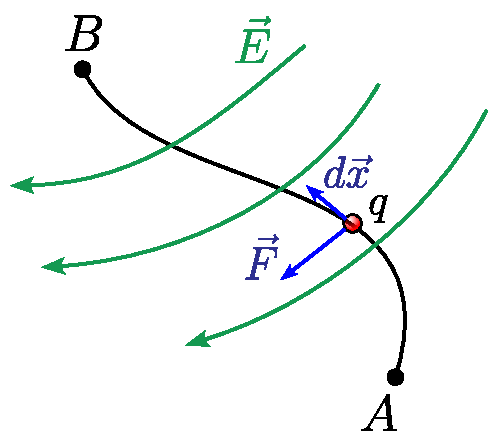
\includegraphics[scale = 0.65]{Figuras/Significado-Potencial.pdf}
    \caption{Interpretación física del potencial.}
    \label{fig:Significado-Potencial}
\end{figure}

La fuerza que actúa sobre la carga en cualquier punto es
$$\vec{F} = q \vec{E}.$$

Entonces, el trabajo efectuado al mover la carga desde $A$ hasta $B$ es 
$$W = - \int_A^B \vec{F} \cdot d\vec{x} = -q \int_A^B \vec{E} \cdot d\vec{x}.$$

El signo menos aparece porque estamos calculando el trabajo hecho sobre la carga  en contra de la acción del campo (trabajo externo). Con la definición \eqref{Relacion-Campo-Potencial}, el trabajo puede ser escrito como
$$W = q \int_A^B \vec{\nabla} \phi \cdot d\vec{x} = q \int_A^B d\phi = q (\phi(B) - \phi(A)).$$

Ésto muestra que $q\phi$ puede ser interpretado como la energía potencial de la carga de prueba en el campo electrostático. 

Finalmente, se tiene una importante relación.
\begin{shaded}
    $$- \int_A^B \vec{E} \cdot d\vec{x} = \phi(B) - \phi(A).$$
\end{shaded}

Se mencionó una energía potencial en el penúltimo párrafo, la cual puede ser asociada a una fuerza conservativa. Por ello, se probará que la fuerza electrostática y por consiguiente el campo electrostático (no dinámico) es conservativo.

Recordemos que
$$\vec{\nabla} \times \vec{E} = \vec{ \nabla} \times (- \vec{\nabla} \phi) = \vec{0}.$$

Usando el teorema de Stokes,
$$\oint_C \vec{E} \cdot d\vec{x} = \iint_S \vec{\nabla} \times \vec{E} \cdot \hat{n} dS = 0,$$

lo cual implica que
$$\oint_C \vec{F} \cdot d\vec{x} = \oint_C q \vec{E} \cdot d\vec{x} = 0.$$

Por lo tanto, $\vec{F}$ es una fuerza conservativa, pues el trabajo realizado en cualquier trayectoria cerrada es cero.

Entonces,
$$W = -\Delta U,$$

donde $U$ es la \textbf{energía potencial eléctrica}.

Por otro lado,
$$-W = -q \int_A^B \vec{E} \cdot d\vec{x} = q \int_A^B \vec{\nabla} \phi \cdot d \vec{x} = \Delta U$$
$$\Rightarrow \qquad \frac{- W}{q} = \int_A^B \vec{\nabla} \phi \cdot d \vec{x} = \frac{\Delta U}{q} = \phi(B) - \phi(A).$$

\newpage
\textbf{Observaciones:}
\begin{enumerate}

\item La diferencia de potencial electrostático lo podemos interpretar como el trabajo realizado para traer una carga desde el punto $A$ hasta el punto $B$ por unidad de carga. 

\item  El potencial electrostático también es llamado \textbf{voltaje} ($V$) y $\Delta V = V_B - V_A$ es la diferencia del voltaje.

\item La unidad de medida es el “Volt”, $1 \,[V] = 1 \, \mbox{Volt} = \frac{1 J}{1C}$.

\item El valor de $\phi$ en una posición no tiene sentido (al igual que en el caso gravitacional, sólo las diferencias de energía potencial tienen significado) a menos que definamos una posición de referencia donde el potencial valga cero. Es usual elegir el punto $A$ en el infinito del tal forma que $\phi(\infty) = 0$. Para así, definir el potencial en un punto $B$ como
$$\phi(B) = - \int_{\infty}^B \vec{E} \cdot d\vec{x}.$$

\textbf{Ojito:} El punto de referencia en el infinito no siempre es una buena elección, por ejemplo, para distribuciones infinitas.

\item No hay que confundir la \textbf{energía potencial electrostática} con \textbf{potencial electrostático}. La energía potencial se mide en \textit{Joule} y es un número único (es trabajo) mientras que el potencial se mide en \textit{Volt} y es diferente en todas partes del espacio.
\end{enumerate}

\section{Potencial eléctrico de cargas puntuales}

El campo eléctrico generado por una carga puntual $q'$ ubicada en el origen está dado por:
$$\Vec{E}(x,y,z) = \frac{1}{4\pi \varepsilon_0} \frac{q'}{(\sqrt{x^2+y^2+z^2})^3} (x \,\hat{\imath} + y \, \hat{\jmath} + z\, \hat{k}).$$

En coordenadas esféricas,
$$\Vec{E}(\Vec{x}) =  \frac{1}{4\pi \varepsilon_0} \frac{q'}{r^2} \, \hat{r}.$$

Como $\vec{E} = - \vec{\nabla} \phi$, se  tiene que
$$\frac{1}{4\pi \varepsilon_0} \frac{q'}{r^2} \, \hat{r} = - \frac{\partial \phi}{\partial r} \,\hat{r} - \frac{1}{r} \frac{\partial \phi}{\partial \theta} \,\hat{\theta} - \frac{1}{r\sin\theta} \frac{\partial \phi}{\partial \varphi} \,\hat{\varphi},$$

donde se escribió el gradiente en coordenadas esféricas. Igualando la componentes, tenemos que
$$\frac{\partial \phi}{\partial r} = -\frac{1}{4\pi \varepsilon_0} \frac{q'}{r^2} \,\wedge\, \frac{\partial \phi}{\partial \theta} = 0 \,\wedge\, \frac{\partial \phi}{\partial \varphi} = 0,$$

es decir, el potencial no depende de $\theta$ y $\varphi$. Entonces, $\phi$ es solo de función de $r$ y por tanto la derivada parcial pasa a escribirse como una derivada ordinaria, ésto es,
$$\frac{d\phi}{dr} =  -\frac{1}{4\pi \varepsilon_0} \frac{q'}{r^2}.$$

Integrando con respecto a $r$,
$$\phi(r) =  \frac{1}{4\pi\varepsilon_0} \frac{q'}{r} + C.$$

Si imponemos que $\phi(\infty) \stackrel{!}{=} 0$, es decir, elegimos como potencial de referencia cero en el infinito, obtenemos que $C = 0$. Luego,
$$\phi(r) =  \frac{1}{4\pi\varepsilon_0} \frac{q'}{r}.$$

Ahora, si consideramos otro sistema coordenado tal que el vector posición de la carga es $\vec{x}\,'$, tenemos que para este sistema, el potencial está dado por
\begin{shaded}
    $$\phi(\Vec{x}) = \frac{1}{4\pi \varepsilon_0} \frac{q'}{|\vec{x} - \Vec{x}\,'|}.$$
\end{shaded}

Podemos interpretar este potencial electrostático como el trabajo que sería realizado sobre una carga $q$ debido a $q'$ para traerla desde el infinito hasta el punto $\Vec{x}$.

Para obtener el potencial eléctrico resultante entre dos o más cargas $q_i$, se aplica el \textit{principio de superposición}. Así, el potencial eléctrico total en $\vec{x}$, es la suma de los potenciales individuales:
\begin{shaded}
    $$\phi(\Vec{x}) = \frac{1}{4\pi \varepsilon_0} \sum_i \frac{q_i}{|\Vec{x} - \Vec{x}_i|},$$
\end{shaded}

donde $\vec{x}_i$ es la posición de la carga $q_i$.

\section{Potencial eléctrico de distribuciones continuas de carga}

Para una distribución continua de carga consideramos un elemento de carga $dq'$ en un volumen $dV'$.

\begin{figure}[H]
    \centering
    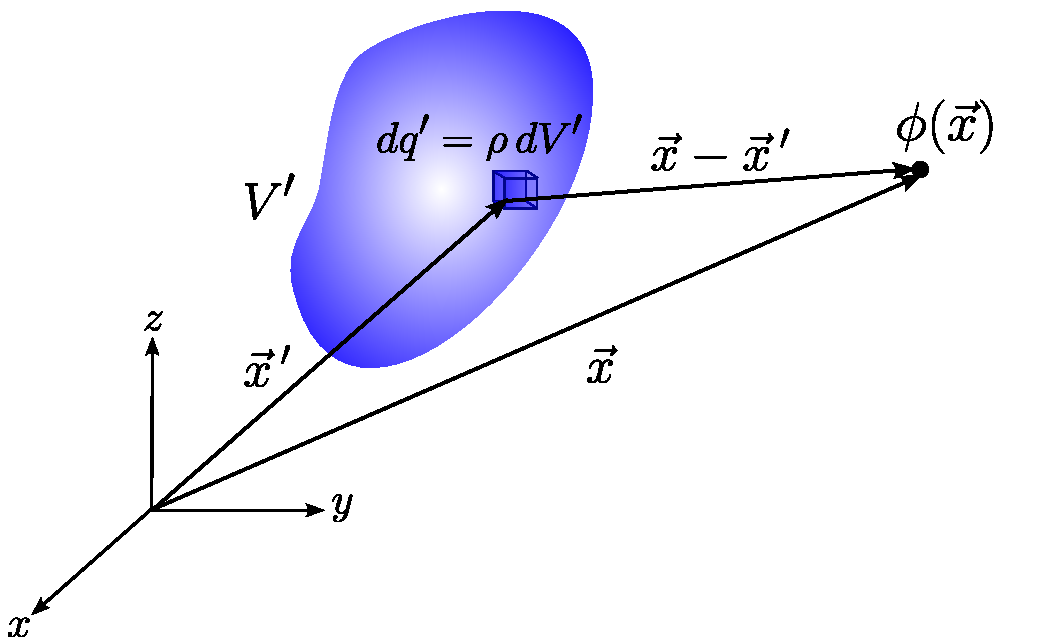
\includegraphics[scale = 0.6]{Figuras/Distribucion-Cargas-Potencial.pdf}
    \caption{Distribución de carga.}
    \label{fig:Distribu-Carga-2}
\end{figure}

El potencial en $\Vec{x}$ debido a $dq'$ es
\begin{equation*}
d\phi = \frac{1}{4\pi\varepsilon_0} \frac{dq'}{|\vec{x} - \vec{x}\,'|}.
\end{equation*}

Integrando en todo el volumen,
\begin{shaded}
\begin{equation}
   \phi(\vec{x}) = \frac{1}{4\pi\varepsilon_0} \iiint_{V'} \frac{dq'}{|\vec{x} - \vec{x}\,'|} = \frac{1}{4\pi\varepsilon_0} \iiint_{V'} \frac{\rho(\vec{x}\,')}{|\vec{x} - \vec{x}\,'|} \,dV'. \label{Potencial-Distri}
\end{equation}
\end{shaded}

En la ecuación \eqref{Potencial-Distri} se supuso que se tenía una distribución volumétrica de carga.

\textbf{Observación:} En la expresión del potencial para una carga puntual o una distribución continua estamos suponiendo que $\phi(\infty) = 0$ (válido para toda distribución finita o compacta), pero hay casos en que esa elección no es posible. Siempre hay que tener en mente que lo que se está calculando, es en realidad una diferencia de potencial:
$$\Delta \phi = \frac{1}{4\pi \varepsilon_0} \int \frac{dq'}{|\vec{x} - \vec{x}\,'|}.$$

\subsection{Aplicaciones del potencial}

\begin{ejemplo}
 Un semianillo de radio $R$ tiene una densidad lineal de carga $\lambda(\varphi) =  \frac{A}{R} \sin \varphi$, con $A = cte$, ver figura \ref{fig:Ej-Potencial-1}. Calcular el potencial electrostático sobre el eje $z$ generado por el semianillo.

\begin{figure}[H]
    \centering
    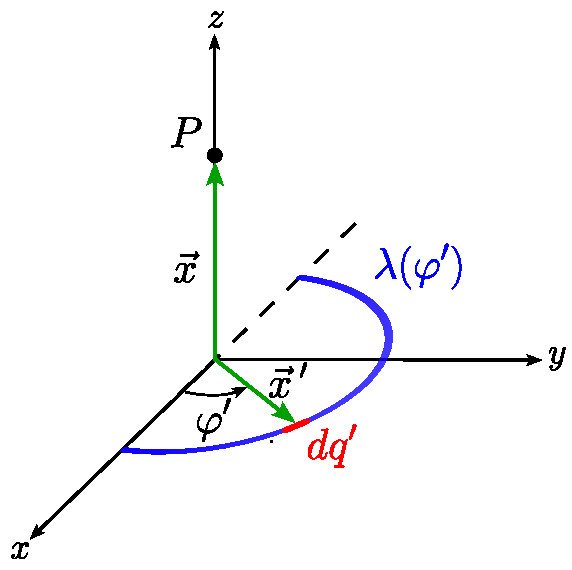
\includegraphics[scale = 0.6]{Figuras/Ej-Potencia-1.pdf}
    \caption{Semianillo de radio $R$ con $\lambda(\varphi) = \frac{A}{R} \sin \varphi$.}
    \label{fig:Ej-Potencial-1}
\end{figure}

\textbf{Solución:} Para calcular el potencial electrostático, se considerará el de referencia cero en el infinito, lo cual es posible ya que la distribución de carga es compacta.

Usando coordenadas cilíndricas, se tiene que
$$dq' = \lambda(\varphi') R \,d\varphi', \quad \vec{x} = z \,\hat{k}, \quad \Vec{x}\,' = R\,\hat{\rho} = R(\cos \varphi'\,\hat{\imath} + \sin \varphi'\,\hat{\jmath}),$$

con $0\leq \varphi' \leq \pi$.

Luego, el diferencial de potencial electrostático en $\vec{x}$ está dado por
\begin{align*}
    d\phi(\Vec{x}) &= \frac{1}{4\pi\varepsilon_0} \frac{dq'}{|\vec{x} - \Vec{x}\,'|} \\
    &= \frac{1}{4\pi\varepsilon_0} \frac{\lambda(\varphi') R}{|z\,\hat{k} - R\,\hat{\rho}|} \,d\varphi' \\
    &= \frac{1}{4\pi\varepsilon_0} \frac{A\sin\varphi'}{\sqrt{z^2 + R^2}} \,d\varphi'.
\end{align*}

Integrando a ambos lados, el potencial electrostático es
\begin{align*}
    \phi(\Vec{x}) &= \int_0^{\pi} \frac{1}{4\pi\varepsilon_0} \frac{A\sin\varphi'}{\sqrt{z^2 + R^2}} \,d\varphi' \\
    &= \frac{1}{4\pi \varepsilon_0} \frac{A}{\sqrt{z^2+R^2}} \int_0^{\pi} \sin \varphi' \,d\varphi' \\
    &= \frac{1}{4\pi \varepsilon_0} \frac{A}{\sqrt{z^2+R^2}} [-\cos\varphi']_0^{\pi} \\
    &=  \frac{1}{2\pi \varepsilon_0} \frac{A}{\sqrt{z^2+R^2}}.
\end{align*}

\end{ejemplo}

\begin{ejemplo} \label{Potencial-Disco}
   Para un disco con densidad de carga constante $\sigma$, radio interior $r$ y radio exterior $R$. Calcule el campo potencial electrostático para el punto $P$, ver figura \ref{fig:Ej-Potencial-2}.

\begin{figure}[H]
    \centering
    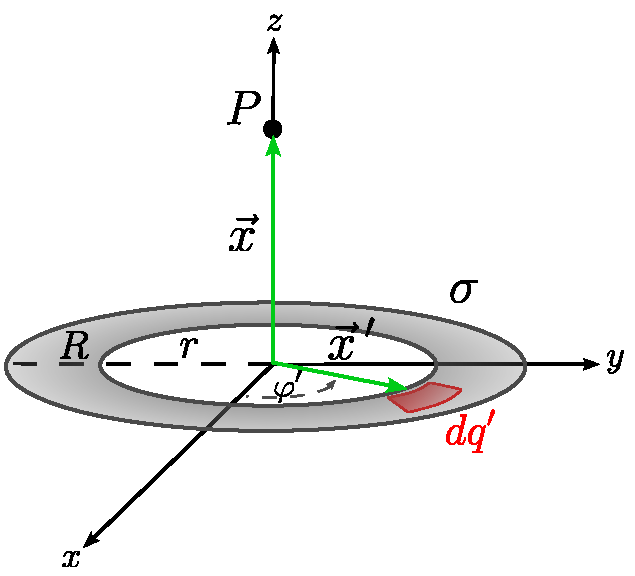
\includegraphics[scale = 0.65]{Figuras/Ej-Potencial-2.pdf}
    \caption{Disco de radio interior $r$ y radio exterior $R$ con densidad de carga $\sigma$ constante.}
    \label{fig:Ej-Potencial-2}
\end{figure}

\textbf{Solución:} Para calcular el potencial electrostático, se considerará el de referencia cero en el infinito, lo cual es posible ya que la distribución de carga es compacta.

Usando coordenadas cilíndricas, se tiene que
$$dq' = \sigma \rho' \,d\varphi'\,d\rho',\quad \Vec{x} = z\,\hat{k}, \quad \Vec{x}\,' = \rho' \, \hat{\rho} = \rho' (\cos \varphi'\,\hat{\imath} + \sin \varphi'\,\hat{\jmath}).$$

Luego, el diferencial de potencial electrostático en $\vec{x}$ está dado por
\begin{align*}
    d\phi(\Vec{x}) &= \frac{1}{4\pi\varepsilon_0} \frac{dq'}{|\vec{x} - \Vec{x}\,'|} \\
    &= \frac{1}{4\pi\varepsilon_0} \frac{\sigma \rho' \,d\varphi'\,d\rho'}{|z\,\hat{k} - \rho' \,\hat{\rho}|}\\
    &= \frac{1}{4\pi\varepsilon_0} \frac{\sigma \rho'}{\sqrt{z^2 + \rho'\,^2}} \,d\varphi'\,d\rho'.
\end{align*}

Integrando a ambos lados, el potencial electrostático es
\begingroup
\allowdisplaybreaks
\begin{align*}
    \phi(\Vec{x}) &= \int_r^R \int_0^{2\pi}  \frac{1}{4\pi\varepsilon_0} \frac{\sigma \rho'}{\sqrt{z^2 + \rho'\,^2}} \,d\varphi'\,d\rho' \\
    &= \frac{\sigma}{4\pi \varepsilon_0} \int_r^R \frac{\rho'}{\sqrt{z^2+\rho'\,^2}} \left(\int_0^{2\pi} d\varphi' \right) d\rho' \\
    &= \frac{2\pi \sigma}{4\pi \varepsilon_0} \int_r^R \frac{\rho'}{\sqrt{z^2+\rho'\,^2}}  d\rho' \\
    &= \frac{\sigma}{2\varepsilon_0} \left[ \sqrt{z^2 + \rho'\,^2}\right]_r^R \\
    &= \frac{\sigma}{2\varepsilon_0} \left( \sqrt{z^2 + R^2} - \sqrt{z^2 + r^2}\right).
\end{align*}
\endgroup
  
\end{ejemplo}

\begin{ejemplo}
Calcule el potencial electrostático para cualquier punto en el espacio de la esfera de radio $R$ y con densidad de carga uniforme e igual a $\rho$.

\textbf{Solución:} En la sección \ref{Ley-Gauss} calculamos el campo electrostático de una esfera de radio $R$ y densidad de carga $\rho$, el cual está dado por:
$$\Vec{E}(r) = \left\{ \begin{array}{cl}
   \frac{\rho R^3 }{3\varepsilon_0 r^2} \,\hat{r},  & \text{si} \quad r > R  \\
    \frac{\rho r}{3\varepsilon_0} \,\hat{r}, & \text{si} \quad  0 \leq r < R 
\end{array} \right. .$$

Para calcular el potencial electrostático, recordemos que 
$$\phi(B) - \phi(A) = - \int_A^B \Vec{E} \cdot d\Vec{x}.$$

Como el campo electrostático es conservativo, la integral de línea no depende del camino de integración, por tanto elegiremos la trayectoria que une a un punto $A$ ubicado al infinito con el punto $B$ cualquiera con coordenada esférica $r$ por medio de  un rayo que parte de $A$ hasta $B$. Luego, $d\Vec{x} = dr'\,\hat{r}$ y
$$\phi(r) - \phi(\infty) = - \int_{\infty}^{r} (E(r') \,\hat{r}) \cdot (dr' \,\hat{r}) = -\int_{\infty}^r E(r') \,dr'.$$

Imponiendo $\phi(\infty) \stackrel{!}{=} 0$,
$$\phi(r) = - \int_{\infty}^r E(r') \,dr'.$$

\begin{itemize}
\item[i)] Si $r > R$, 
\begin{align*}
    \phi(r) = - \int_{\infty}^r E(r') \,dr' 
    &= - \int_{\infty}^r \frac{\rho R^3 }{3 \varepsilon_0 r'\,^2} \,  dr' \\
&= - \frac{\rho R^3}{3\varepsilon_0} \int_{\infty}^r \frac{1}{r'\,^2}\, dr' \\
&= - \frac{\rho R^3}{3\varepsilon_0} \left[ - \frac{1}{r'} \right]_{\infty}^r \\
&= \frac{\rho R^3}{3\varepsilon_0 r}.
\end{align*}

\item[ii)] Si $0 \leq r  < R$, 
\begin{align*}
    \phi(r) &= - \int_{\infty}^r E(r') \,dr' \\
    & = - \int_{\infty}^R \frac{\rho R^3}{3 \varepsilon_0 r'\,^2} \, dr' - \int_{R}^r \frac{\rho r'}{3 \varepsilon_0} dr' \\
&= - \frac{\rho R^3 }{3\varepsilon_0} \int_{\infty}^R \frac{1}{r'\,^2} \,dr' - \frac{\rho}{3\varepsilon_0} \int_R^r r' \,dr' \\
&= - \frac{\rho R^3}{3\varepsilon_0} \left[ -\frac{1}{r'} \right]_{\infty}^R - \frac{\rho}{3\varepsilon_0} \left[ \frac{1}{2}r'\,^2 \right]_R^r \\
&= \frac{\rho R^3}{3\varepsilon_0 R} - \frac{\rho}{3\varepsilon_0} \left( \frac{r^2}{2} - \frac{R^2}{2} \right) \\
&= \frac{\rho}{6 \varepsilon_0}(3R^2 - r^2).
\end{align*}

Por lo tanto,
\begin{equation*}
\phi(r) =  \left\{ \begin{array}{cl}
   \frac{\rho R^3 }{3\varepsilon_0 r} ,  & \text{si} \quad r > R  \\
    \frac{\rho}{6\varepsilon_0} (3R^2-r^2), & \text{si} \quad  0 \leq r < R 
\end{array} \right. .
\end{equation*}

\end{itemize}
\end{ejemplo}

\begin{ejemplo}\label{Potencial-Plano-Inf}
     Calcule el potencial electrostático a una distancia $d$, generado por un plano infinito con densidad de carga uniforme y de valor $\sigma$.

\textbf{Solución:} En este caso no podemos asumir que el potencial es cero en el infinito, pues el campo no es débil en el infinito como en el caso de las distribuciones de carga compactas. De hecho, si usamos el potencial de un disco  finito del ejemplo \ref{Potencial-Disco} y tomamos $r = 0$ y el límite cuando $R$ tiende al infinito:
$$\lim_{R \to \infty} \frac{\sigma}{2\varepsilon_0} \left( \sqrt{z^2 + R^2} - z \right) = \infty,$$

es decir, esta ecuación no puede ser usada.

Si consideramos el plano infinito en el plano $xy$, el campo eléctrico está dado por:
\begin{equation*}
\Vec{E}(\Vec{x}) =  \left\{ \begin{array}{cl}
   \frac{\sigma}{2 \varepsilon_0} \,\hat{k} ,  & \text{si} \quad z > 0  \\
    - \frac{\sigma}{2 \varepsilon_0} \,\hat{k}, & \text{si} \quad  z < 0 
\end{array} \right. .
\end{equation*}

De nuevo, para calcular el potencial electrostático, recordemos que
$$\phi(B) - \phi(A) = - \int_A^B \Vec{E} \cdot d\Vec{x}.$$

Elegimos como trayectoria aquella que une al punto $A$ con coordenada $d' \geq 0$ en el eje $z$ mediante un segmento con el punto $B$ con coordenada $z$ igual a $d > 0$. Luego, $d\Vec{x} = dz\,\hat{k}$ y
$$\phi(d) - \phi(d') = - \int_{d'}^{d} (E\,\hat{k}) \cdot (dz\,\hat{k}) = - \int_{d'}^d \frac{\sigma}{2\varepsilon_0} \,dz = - \frac{\sigma}{2\varepsilon}(d-d').$$

Si imponemos, por ejemplo, $\phi(d') \stackrel{!}{=} 0$ en $d' = 0$, tenemos que
$$\phi(d) = - \frac{\sigma}{2\varepsilon_0} d.$$

Si $B$ es un punto con coordenada $z$ igual a $-d$, 
$$\phi(-d)= \frac{\sigma}{2\varepsilon_0} d.$$

Por lo tanto, generalizando para todo punto con coordenada $z$ en el espacio,
$$\phi(z) = - \frac{\sigma}{2\varepsilon_0}|z|.$$

\end{ejemplo}

\subsection{Continuidad de los campos}

En la figura \ref{fig:Campo-Plano-Inf}, están representadas las gráficas del campo eléctrico (sin considerar dirección) y el potencial del plano infinito dados por el ejemplo \ref{Potencial-Plano-Inf}.

    \begin{figure}[H]
        \centering
        \subfigure[]{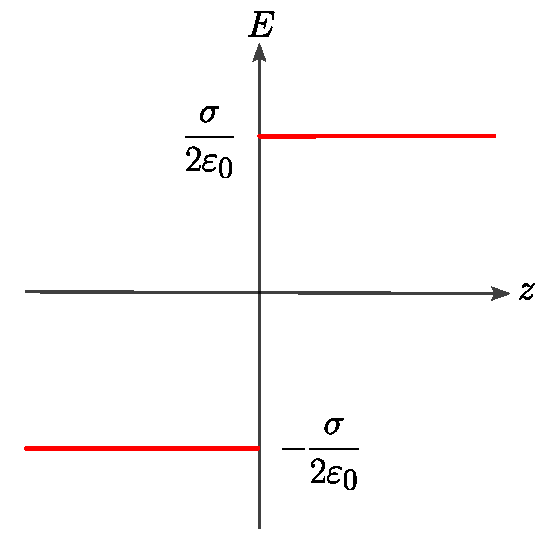
\includegraphics[width=0.4
        \textwidth]{Figuras/Campo-E-Plano.pdf}} \hspace{1cm}
        \subfigure[]{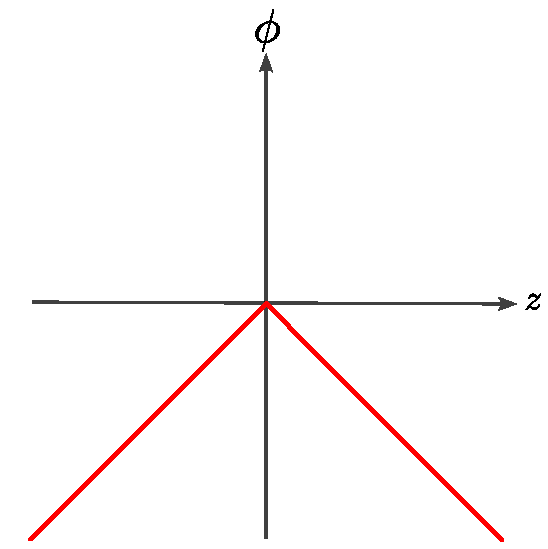
\includegraphics[width=0.4\textwidth]{Figuras/Potencial-Plano.pdf}} 
        \caption{Gráficas del campo eléctrico (a) y el potencial (b) del plano infinito.}
        \label{fig:Campo-Plano-Inf}
    \end{figure}

Claramente el campo eléctrico presenta una discontinuidad en $z = 0$, es decir, donde se ubica la distribución superficial de carga. Sin embargo, el potencial es continuo en todo el espacio.  

En general, el campo eléctrico y el potencial son continuos para toda distribución volumétrica de carga con densidad $\rho(\Vec{x})$ (finita y continua). Sin embargo, si consideramos distribuciones superficiales de carga ($\rho$ discontinua y divergente), el campo eléctrico tenderá a ser discontinuo en la región donde se ubica la distribución superficial de carga (donde $\rho$ es discontinuo), pero finito en el resto de los puntos del espacio. En cambio el potencial seguirá siendo continuo. En el caso de que la distribución de carga se modele incluyendo cargas puntuales o líneas de carga, el potencial ya no será finito en todo punto.

\section{Energía potencial electrostática}

Consideremos un sistema formado por una carga puntual $q_1$ con vector posición $\Vec{x}_1$, ver figura \ref{fig:Energía-Potencial}-(a). Queremos traer (desde el infinito) una carga puntual $q_2$ hasta la posición $\Vec{x}_2$, para ello debemos efectuar un trabajo en contra del campo eléctrico creado por $q_1$, que está dado por \footnote{Recuerde que $\Delta U = q \Delta \phi$ y hemos supuesto que el cero potencial en el infinito.}
$$U = q_2 \phi_1(\Vec{x}_2) = \frac{1}{4\pi\varepsilon_0}\frac{q_1 q_2}{|\Vec{x}_2 - \Vec{x}_1|},$$

donde $\phi_1$ es el potencial debido a la carga $q_1$.

\textbf{Nota:} Si las cargas tienen igual signo, $U > 0$ y corresponderá a la energía invertida para armar el sistema,  la cual será almacenada y al desarmar el sistema esta será la energía liberada. Por otro lado, si las cargas tienen signos opuestos, $U < 0$ y corresponderá a la energía que se necesitará para desarmar el sistema.

Ahora, si traemos (desde el infinito) otra carga puntual $q_3$ hasta la posición $\Vec{x}_3$, ver figura \ref{fig:Energía-Potencial}, la energía potencial será
$$U_3 = q_3 \phi_1(\vec{x_3}) + q_3 \phi_2(\Vec{x}_3) = \frac{1}{4\pi\varepsilon_0}\frac{q_1 q_3}{|\Vec{x}_3 - \Vec{x}_1|} + \frac{1}{4\pi\varepsilon_0}\frac{q_2 q_3}{|\Vec{x}_3 - \Vec{x}_2|}.$$

Luego, la energía potencial almacenada en el sistema es:
$$U = \frac{1}{4\pi \varepsilon_0} \left(\frac{q_1 q_2}{|\Vec{x}_2 - \Vec{x}_1|} + \frac{q_1q_3}{|\Vec{x}_3-\Vec{x}_1| } + \frac{q_2 q_3}{|\Vec{x}_3 - \Vec{x}_2|} \right).$$

Podemos reescribir la expresión anterior de la forma
\begin{align*}
    U &= \frac{1}{2} \left[q_1 \left( \frac{1}{4\pi \varepsilon_0} \frac{q_2}{|\Vec{x}_2-\Vec{x}_1|} + \frac{1}{4\pi \varepsilon_0} \frac{q_3}{|\Vec{x}_3-\Vec{x}_1|} \right) + q_2 \left( \frac{1}{4\pi \varepsilon_0} \frac{q_1}{|\Vec{x}_1-\Vec{x}_2|} + \frac{1}{4\pi \varepsilon_0} \frac{q_3}{|\Vec{x}_3-\Vec{x}_2|} \right) \right. \\
    &\quad \left. + q_3 \left( \frac{1}{4\pi \varepsilon_0} \frac{q_1}{|\Vec{x}_1-\Vec{x}_3|} + \frac{1}{4\pi \varepsilon_0} \frac{q_2}{|\Vec{x}_2-\Vec{x}_3|} \right) \right].
\end{align*}

\begin{figure}[H]
    \centering
    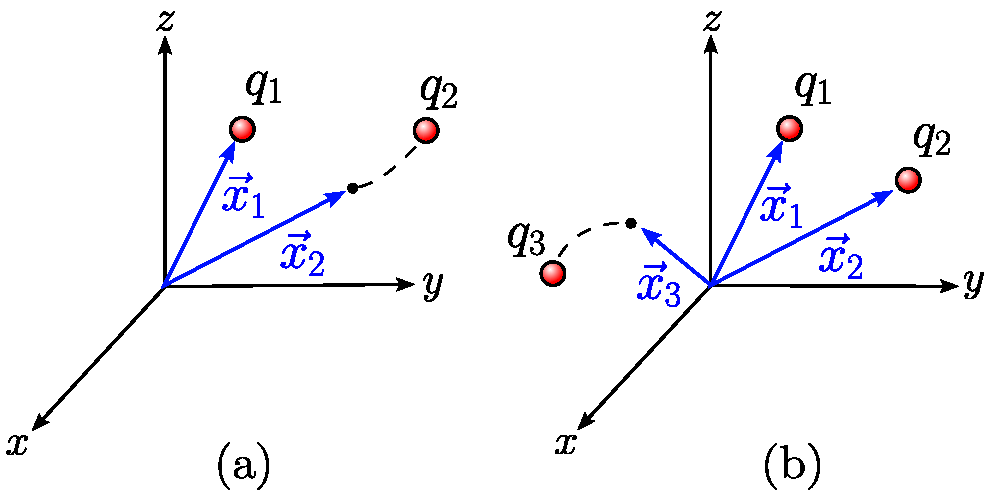
\includegraphics[scale = 0.65]{Figuras/Energia-Potencial.pdf}
    \caption{Construcción de una configuración de cargas empezando con una carga $q_1$, añadiendo luego una carga $q_2$ (a) y una carga $q_3$ (b).}
    \label{fig:Energía-Potencial}
\end{figure}

Generalizando para $n$ cargas:
\begin{shaded}
  $$U = \frac{1}{2} \sum_{i,j (i\neq j)}^n \frac{1}{4\pi \varepsilon_0} \frac{q_i q_j}{|\Vec{x}_j - \Vec{x}_i|} = \frac{1}{2} \sum_{i,j (i\neq j)}^n q_i \phi_i(\Vec{x}_j),$$ 
\end{shaded}

donde  $\phi_i(\Vec{x}_j)$ es el potencial electrostático en el punto donde se sitúa la carga $q_j$ debido a la carga $q_i$ .

En el caso de una \textit{distribución continua de carga}, la energía potencial almacenada (energía de formación) está dada por:
\begin{shaded}
   $$ U = \frac{1}{2} \iiint_{V} \phi(\Vec{x}) \,dq = \frac{1}{2} \iiint_{V} \rho(\Vec{x}) \phi(\Vec{x}) \,dV, $$
\end{shaded}

donde se ha supuesto una distribución volumétrica de carga.

\begin{ejemplo}
    Encontrar la energía necesaria para formar una esfera de carga total $Q$, de radio $R$ y densidad volumétrica de carga constante $\rho$.

\textbf{Solución:} De la sección anterior, se tiene que el potencial electrostático en un punto dentro de la esfera está dado por:
$$\phi(r)= \frac{\rho}{6 \varepsilon_0}(3R^2 - r^2), \quad 0 \leq r \leq R. $$

Como $\rho = cte$,
$$Q = \rho V = \frac{4}{3} \pi R^3 \rho \Rightarrow  \rho = \frac{3 Q}{4\pi R^3}.$$

Luego,
$$\phi(r)= \frac{Q(3R^2-r^2)}{8 \pi \varepsilon_0R^3}, \quad 0 \leq r \leq R. $$

Usando coordenadas esféricas, se tiene que
$$dV = r^2 \sin \theta \,d\varphi\,d\theta\,dr.$$

Por lo tanto, la energía de formación está dada por
\begin{align*}
    U &= \frac{1}{2} \iiint_V \phi(\Vec{x}) \rho \,dV \\
    &= \frac{1}{2} \rho \int_0^R \int_0^{\pi} \int_0^{2\pi} \frac{Q(3R^2-r^2)}{8 \pi \varepsilon_0 R^3} r^2 \sin \theta \,d\varphi \,d\theta\, dr\\
    &= \frac{Q \rho}{16 \pi \varepsilon_0 R^3} \int_0^R (3R^2 - r^2)r^2 \left(  \int_0^{\pi} \sin \theta \left( \int_0^{2\pi} d\varphi \right) d\theta \right) dr \\
    &=  \frac{2\pi Q \rho}{16 \pi \varepsilon_0 R^3} \int_0^R 3 R^2r^2-r^4 \left( \int_0^{\pi} \sin \theta d\theta  \right) dr \\
    &= \frac{Q \rho}{8 \varepsilon_0 R^3} \int_0^R (3R^2 r^2 -r^4) [- \cos\theta]_0^{\pi} dr \\
&= \frac{Q \rho}{4\varepsilon_0 R^3} \int_0^R 3R^2r^2-r^4 dr \\
&=  \frac{Q \rho}{4\varepsilon_0 R^3} \left[ R^2r^3 - \frac{r^5}{5}  \right]_0^R \\
&= \frac{Q \rho}{4 \varepsilon_0 R^3} \left( R^5 - \frac{R^5}{5}  \right) \\
&= \frac{Q \rho R^2}{5 \varepsilon_0}.
\end{align*}

Reemplazando $\rho = \frac{3 Q}{4\pi R^3}$,
$$U = \frac{3 Q^2}{20 \pi \varepsilon_0 R}.$$
\end{ejemplo}


\section{Superficies equipotenciales}

Tal como las líneas de un campo vectorial proporcionan una manera apropiada de visualizar el campo electroestático para una distribución de cargas, el potencial electroestático en diversos puntos se puede representar gráficamente mediante \textbf{superficies equipotenciales}.

En general:

\begin{itemize}
\item[i)] Las superficies equipotenciales son aquellas en las que todos sus puntos tienen el mismo potencial. En otras palabras,
$$\Delta \phi = 0.$$

Además, puesto que $\Delta U = q \Delta \Phi$, no se efectúa trabajo para mover una partícula cargada $q$ entre dos puntos de la misma superficie equipotencial.

\item[ii)] El campo electroestático $\vec{E}$ es perpendicular a la superficie equipotencial.

En efecto, de la expresión $\phi(B) - \phi(A) = - \int_A^B \vec{E} \cdot d\vec{x}$ podemos decir que cuando una carga efectúa un desplazamiento infinitesimal $d\vec{x}$ a lo largo de una superficie equipotencial, entonces
$$d\phi = \vec{E} \cdot d\vec{x} = 0 \Rightarrow \vec{E} \perp d\vec{x}.$$
\end{itemize} 

\begin{ejemplo}
    Considere dos cargas puntuales $q_1$ y $q_2$, con vectores posición $\Vec{x}_1$ y $\Vec{x}_2$, respectivamente. Encuentre las superficies equipotenciales.

    \textbf{Solución:}  El potencial electroestático en un punto $\Vec{x}$ está dado por
$$\phi(\Vec{x}) = \phi_1(\Vec{x}) + \phi_2(\Vec{x}) = \frac{1}{4\pi\varepsilon_0} \frac{q_1}{|\Vec{x} - \vec{x}_1|} + \frac{1}{4\pi\varepsilon_0} \frac{q_2}{|\Vec{x} - \vec{x}_2|}.$$

Usando coordenadas cartesianas, 
$$\Vec{x} = (x,y,z), \quad \Vec{x}_1 = (x_1,y_1,z_1), \quad \Vec{x}_2 = (x_2,y_2,z_2).$$

\begin{itemize}
\item \textbf{Caso 1}: $q_2 = 0$,
$$\phi = \frac{1}{4\pi\varepsilon_0} \frac{q_1}{\sqrt{(x-x_1)^2 + (y-y_1)^2  + (z-z_1)^2}}.$$

Para encontrar la superficie equipotencial tomemos $\phi = \phi_0 \neq 0$ constante.
$$(x-x_1)^2 + (y-y_1)^2 + (z-z_1)^2 = \left( \frac{1}{4\pi\varepsilon_0} \frac{q_1}{\phi_0} \right)^2.$$

Por lo tanto, las superficies equipotenciales para una carga puntual $q_1$ son esferas centradas en $(x_1,y_1,z_1)$ y radio $q_1/(4\pi\varepsilon_0 \phi_0)$. 

\item \textbf{Caso 2}: Si $q_1 = q_2 \neq 0$, la ecuación que define la superficie está dada por:
\begin{equation*}
 \frac{q_1}{\sqrt{(x-x_1)^2 + (y-y_1)^2  + (z-z_1)^2}} + \frac{q_2}{\sqrt{(x-x_2)^2 + (y-y_2)^2  + (z-z_2)^2}} = cte.
\end{equation*}
\end{itemize}
\end{ejemplo}

En la  figura \ref{fig:SuperficiesEquipotenciales}, las líneas azules corresponden a superficies equipotenciales. En \textcolor{red}{a)} las líneas de campo radiales y las superficies equipotenciales son esferas concéntricas. En \textcolor{red}{b)} y \textcolor{red}{c)} vemos superficies equipotenciales de dos cargas.


\begin{figure}[H]
        \centering
        \subfigure[]{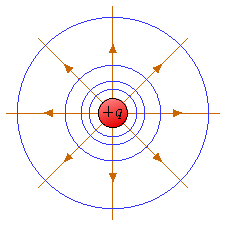
\includegraphics[width=0.37\textwidth]{Figuras/Equipotencial-Carga+.pdf}} \hspace{1cm}
        \subfigure[]{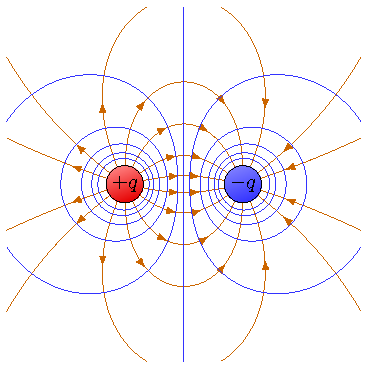
\includegraphics[width=0.37\textwidth]{Figuras/Equipotencial-Carga+-.pdf}} 
        \hspace{1cm}
        \subfigure[]{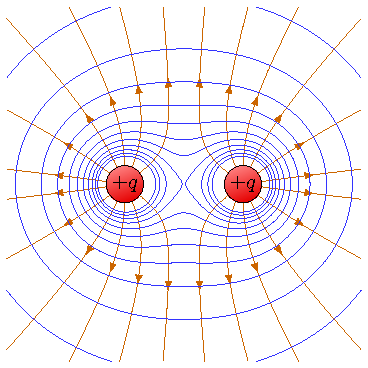
\includegraphics[width=0.37\textwidth]{Figuras/Equipotencial-Carga++.pdf}} 
        \caption{Campo eléctrico y superficies equipotenciales de una carga puntual positiva (a), de dos cargas con signos opuestos (b) y dos cargas positivas (c). Recuperado de: \href{https://tikz.net/electric_fieldlines2/}{tikz.net}. } \label{fig:SuperficiesEquipotenciales}
    \end{figure}


\section{Ecuación de Poisson y Laplace*}

De la forma diferencial de la ley de Gauss:
$$\Vec{\nabla} \cdot \Vec{E} = \frac{\rho(\Vec{x})}{\varepsilon_0}$$

y recordando que (en electrostática) $\Vec{E} = - \Vec{\nabla} \phi$, podemos combinar estos dos términos
$$\Vec{\nabla} \cdot (- \Vec{\nabla} \phi) = - (\Vec{\nabla} \cdot\Vec{\nabla} ) \phi = \frac{\rho(\Vec{x})}{\varepsilon_0}.$$

Pero, $\Vec{\nabla} \cdot\Vec{\nabla} = \nabla^2$ es el laplaciano. Entonces, el potencial electrostático satisface la \textbf{ecuación de Poisson}
\begin{shaded}
    $$\nabla^2 \phi = - \frac{\rho}{\varepsilon_0}.$$
\end{shaded}

En regiones del espacio donde no se encuentren distribuciones de carga, $\rho \equiv 0$, el potencial satisface la \textbf{ecuación de Laplace}:
\begin{shaded}
    $$\nabla^2 \phi = 0.$$
\end{shaded}

Para resolver cualquiera de las ecuaciones diferenciales, tendremos que hacer consideraciones de simetría, expresar el laplaciano en un sistema coordenado adecuado para facilitar los cálculos y plantear condiciones de borde.

\begin{ejemplo}
    Considere dos cilindros coaxiales muy largos, a diferente potencial, ver figura \ref{fig:CilindrosCoaxiales}. Encontrar el potencial entre los cilindros y el campo eléctrico.

    \begin{figure}[H]
        \centering
        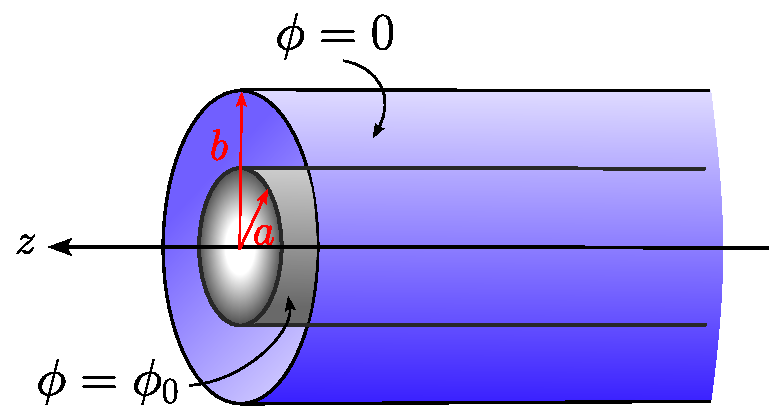
\includegraphics[scale = 0.65]{Figuras/Ej-EcLaplace.pdf}
        \caption{Cilindros coaxiales.}
        \label{fig:CilindrosCoaxiales}
    \end{figure}

    \textbf{Solución:} Dado que los cilindros son extensos bajo un potencial constante, tenemos simetría de traslación con respecto al eje $z$ y simetría de rotación con respecto al eje $z$. Entonces, el potencial no depende de $\varphi$ ni de $z$. La ecuación de Laplace en coordenada cilíndricas es
    $$\nabla^2 \phi = \frac{1}{\rho} \frac{\partial}{\partial \rho}\left(\rho \frac{\partial \phi}{\partial \rho} \right) + \frac{1}{r^2} \frac{\partial^2 \phi}{\partial \varphi^2} + \frac{\partial^2 \phi}{\partial z^2} = 0,$$

    la cual queda reducida a
    $$\frac{1}{\rho} \frac{d}{d\rho}\left( \rho \frac{d \phi}{d\rho} \right) = 0.$$

    Integrando dos veces con respecto a $\rho$, tenemos que
    $$\rho \frac{d\phi}{d\rho} = C_1 \Rightarrow \frac{d \phi}{d\rho} = \frac{A}{\rho} \Rightarrow \phi(\rho) = C_1 \ln(\rho) + C_2,$$

    donde $C_1$ y $C_2$ son constantes de integración. Si imponemos las condiciones de borde: $\phi(a) = \phi_0$ y $\phi(b) = 0$, encontramos que
    $$C_1 = - \phi_0\frac{1}{\ln(b/a)}~\text{y}~ C_2 = \phi_0 \frac{\ln(b)}{\ln(b/a)}.$$

    Por lo tanto,
    $$\phi(\rho) = \phi_0 \frac{\ln(b/\rho)}{\ln(b/a)}.$$

    El campo eléctrico está dado por
    $$\Vec{E} = - \Vec{\nabla} \phi = - \left( \frac{\partial \phi}{\partial \rho} \,\hat{\rho} + \frac{1}{\rho} \frac{\partial \phi}{\partial \varphi} \,\hat{\varphi} + \frac{\partial \phi}{\partial z}\,\hat{k} \right) = \frac{\phi_0}{\rho \ln(b/a)} \,\hat{\rho}.$$
\end{ejemplo}

\section{El momento dipolar eléctrico}

Un \textbf{dipolo eléctrico} es un sistema formado por dos cargas puntuales iguales y de signo contrario y fijas a una distancia $d$. Consideremos entonces dos cargas $+q$ y $-q$ con vectores posición $\Vec{x}_1 = (d/2) \,\hat{k}$ y $\Vec{x}_2 = -(d/2)\,\hat{k}$, ver figura \ref{fig:dipolo}.

El potencial en todo punto del espacio está dado por
$$\phi(\Vec{x}) = \frac{q}{4\pi\varepsilon_0} \left( \frac{1}{|\Vec{x} - \Vec{x}_1|} - \frac{1}{|\Vec{x} - \Vec{x}_2|}\right).$$

Usando coordenadas esféricas, $\Vec{x} = r \,\hat{r} = r(\sin \theta \cos\varphi \,\hat{\imath} + \sin \theta \sin \varphi\,\hat{\jmath} + \cos \theta \,\hat{k})$, tenemos que \footnote{Se obtiene el mismo resultado aplicando el teorema del coseno.}
\begingroup
\allowdisplaybreaks
\begin{align*}
    |\Vec{x} - \Vec{x}_1| &= \sqrt{\left(r\,\hat{r} - \frac{d}{2} \,\hat{k} \right) \cdot\left(r\,\hat{r} - \frac{d}{2} \,\hat{k} \right) } \\
    &= \sqrt{r^2 + \left(\frac{d}{2} \right)^2 - 2 r \left( \frac{d}{2} \right) \hat{r} \cdot \hat{k}} \\
    &= \sqrt{r^2 + \left(\frac{d}{2} \right)^2 - rd \cos\theta} ,\\
     |\Vec{x} - \Vec{x}_2| &= \sqrt{\left(r\,\hat{r} + \frac{d}{2} \,\hat{k} \right) \cdot\left(r\,\hat{r} + \frac{d}{2} \,\hat{k} \right) } \\
    &= \sqrt{r^2 + \left(\frac{d}{2} \right)^2 + 2 r \left( \frac{d}{2} \right) \hat{r} \cdot \hat{k}} \\
    &= \sqrt{r^2 + \left(\frac{d}{2} \right)^2 + rd \cos\theta} .
\end{align*}
\endgroup


Luego, nuestro potencial nos queda
\begin{equation}
  \phi(r,\theta) = \frac{q}{4\pi\varepsilon_0} \left(\frac{1}{\sqrt{r^2 + \left(\frac{d}{2} \right)^2 - rd \cos\theta}} - \frac{1}{\sqrt{r^2 + \left(\frac{d}{2} \right)^2 + rd \cos\theta}} \right). \label{PotencialDipolo}  
\end{equation}

\begin{figure}[H]
    \centering
    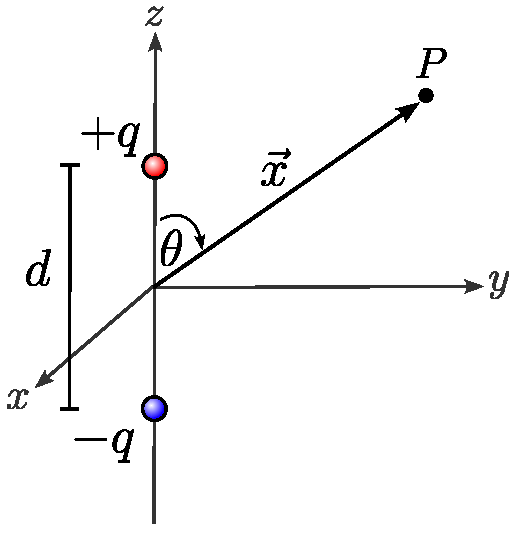
\includegraphics[scale = 0.7]{Figuras/DipoloElectrico.pdf}
    \caption{Dipolo eléctrico.}
    \label{fig:dipolo}
\end{figure}

Nos interesa tomar el límite cuando $d \to 0$. Sea la función 
$$f(d) = \frac{1}{\sqrt{r^2 + \left(\frac{d}{2} \right)^2 - rd \cos\theta}}, \quad \text{para} ~ d \ll 1,$$

expandamos en serie de Taylor alrededor de $d = 0$ para $d \ll 1$:
\begin{align*}
    f(d) &= f(0) + f'(0) d + \mathcal{O}(d^2) \\
    &= \frac{1}{r} - \frac{1}{2r^3} (-r \cos\theta) d + \mathcal{O}(d^2) \\
    &= \frac{1}{r} + \frac{d}{2r^2} \cos \theta + \mathcal{O}(d^2) .
\end{align*}

\textbf{Notación:} $\mathcal{O}(d^2)$ significa que los sumando restantes son proporcionales a $d^2$.

Similarmente,
$$\frac{1}{\sqrt{r^2 + \left(\frac{d}{2} \right)^2 + rd \cos\theta}} = \frac{1}{r} - \frac{d}{2r^2} \cos\theta + \mathcal{O}(d^2).$$

Reemplazando en \eqref{PotencialDipolo},
\begin{align*}
   \phi(r, \theta) &= \frac{q}{4\pi\varepsilon}  \left( \frac{1}{r} + \frac{d}{2r^2} \cos \theta - \frac{1}{r} +  \frac{d}{2r^2} \cos \theta \mathcal{O}(d^2) \right) \\
   &= \frac{q}{4\pi \varepsilon_0} \frac{d}{r^2} \cos \theta + \mathcal{O}(qd^2).
\end{align*}

Tomando los límites: $d\to 0$ y $q \to \infty$ tal que $d\cdot q$ sea finito, encontramos que 
$$\phi(r,\theta) \to  \frac{1}{4\pi \varepsilon_0} \frac{qd}{r^2} \cos \theta.$$

La configuración de cargas, bajo estos límites, se conoce como \textbf{dipolo eléctrico ideal} y si definimos el \textbf{momento dipolar eléctrico} como el vector 
$$\Vec{p} := q \Vec{d},$$

donde $\vec{d}$ es un vector de módulo $d$ que va desde la carga negativa a la positiva, tenemos que el potencial del dipolo ideal está dado por
\begin{shaded}
\begin{equation}
   \phi_{dip}(r,\theta) = \frac{p}{4\pi \varepsilon_0} \frac{\cos \theta}{r^2} = \frac{1}{4\pi \varepsilon_0} \frac{\vec{p} \cdot \hat{r}}{r^2}. \label{Potencial-Dipolo-Ideal}
\end{equation}
\end{shaded}

Para obtener el campo eléctrico producido por el dipolo, usaremos el gradiente en coordenadas esféricas.
\begin{align*}
    \Vec{E} &= - \vec{\nabla} \phi \\
    &= - \left( \frac{\partial \phi}{\partial r} \, \hat{r} +  \frac{1}{r} \frac{\partial \phi}{\partial \theta} \, \hat{\theta} + \frac{1}{r\sin\theta} \frac{\partial \phi}{\partial \varphi} \,\hat{\varphi} \right) \\
    &= \frac{1}{4\pi \varepsilon_0} \left(\frac{2p \cos\theta}{r^3} \,\hat{r} + \frac{p \sin\theta}{r^3} \,\theta \right).
\end{align*}

A partir de la figura \ref{fig:MomentoDipolar}, se desprenden las siguientes relaciones:
$$p \cos \theta\,\hat{r} = (\Vec{p} \cdot \hat{r}) \,\hat{r}, \quad p \sin \theta\,\hat{\theta} = - (\Vec{p} - p\cos\theta \,\hat{r}).$$

\begin{figure}[H]
    \centering
    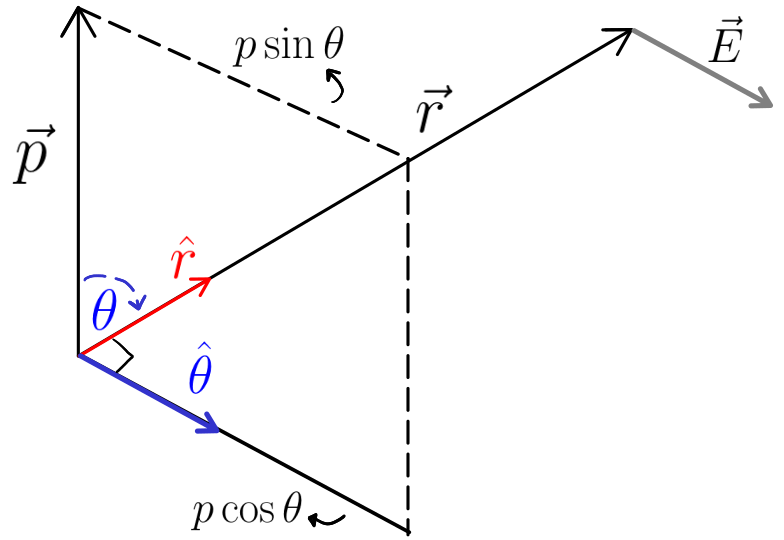
\includegraphics[scale = 0.3]{Figuras/MOmentoDIpolar2.png}
    \caption{Momento dipolar.}
    \label{fig:MomentoDipolar}
\end{figure}

Luego,
\begin{align*}
    \Vec{E} &= \frac{1}{4\pi \varepsilon_0} \frac{1}{r^3} \left(2(\Vec{p} \cdot \hat{r}) \,\hat{r} - (\Vec{p} - p \cos \theta \,\hat{r})  \right) \\
    &=\frac{1}{4\pi \varepsilon_0} \frac{1}{r^3} \left(2(\Vec{p} \cdot \hat{r}) \,\hat{r} - (\Vec{p} - (\Vec{p} \cdot \hat{r}) \,\hat{r})  \right) \\
    &= \frac{1}{4\pi\varepsilon_0} \frac{3(\Vec{p} \cdot \hat{r}) \,\hat{r} - \Vec{p}}{r^3}.
\end{align*}

Por lo tanto, el campo eléctrico de un dipolo ideal está dado por
\begin{shaded}
    $$\Vec{E} = \frac{1}{4\pi \varepsilon_0} \frac{2p \cos\theta\,\hat{r} + p\sin\theta\,\hat{\theta}}{r^3} = \frac{1}{4\pi\varepsilon_0} \frac{3(\Vec{p} \cdot \hat{r}) \,\hat{r} - \Vec{p}}{r^3}.$$
\end{shaded}

\textbf{Observación:} El análisis hecho consideró que la distancia entre las cargas tendía a cero. Queda como ejercicio para el lector verificar que se obtiene el mismo resultado si evaluamos el potencial y el campo eléctrico del dipolo (no ideal) muy lejos, en particular, $d/r \ll 1$. En otras palabras, el dipolo se aproxima a un dipolo ideal muy lejos.

\textbf{Hint:} Expandir en serie de Taylor alrededor de $(d/r) = 0$  la función
$$f\left( \frac{d}{r}\right) = \frac{1}{r\sqrt{1 + \left( \frac{d}{2r}\right)^2 - \frac{d}{r} \cos\theta}}, \quad \text{para} ~ \frac{d}{r} \ll 1.$$

Por último, calculemos el torque sobre un dipolo en un campo externo uniforme.

De la mecánica, sabemos que el torque está dado por $\vec{\tau} = \vec{x} \times \vec{F}$. En el caso del dipolo, se ve que las fuerzas forman una pareja, ver figura \ref{fig:Torque}, de modo que podemos tomar el torque con respecto a $-q$.

\begin{figure}[H]
    \centering
    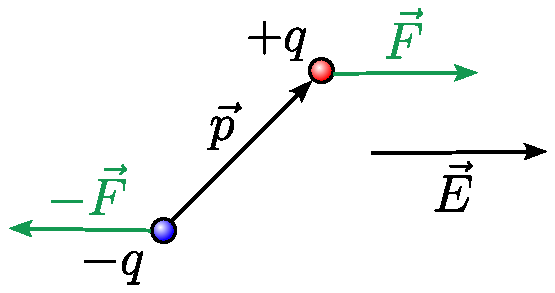
\includegraphics[scale = 0.7]{Figuras/TorqueDipolo.pdf}
    \caption{Torque de un dipolo.}
    \label{fig:Torque}
\end{figure}

Así, podemos escribir
\begin{shaded}
    $$\vec{\tau} = \vec{d} \times q \vec{E} = q\vec{d} \times \vec{E} = \vec{p} \times \vec{E}.$$
\end{shaded}

\section{Conductores}

Entenderemos por \textbf{conductor}, un material que posee movilidad de un número alto de cargas eléctricas que se encuentran en su interior. Si aplicamos un campo eléctrico sobre este tipo de materiales, estas cargas se pueden mover por el interior del material.

Ahora vamos a examinar un caso especial cuando las cargas en el conductor no se mueven, es decir, están en \textbf{equilibrio electrostático}. Para lograr ésto, se establece que en un conductor (cargado), las cargas (en exceso) se distribuyen de tal manera de reducir la repulsión entre ellas.

\begin{figure}[H]
    \centering
    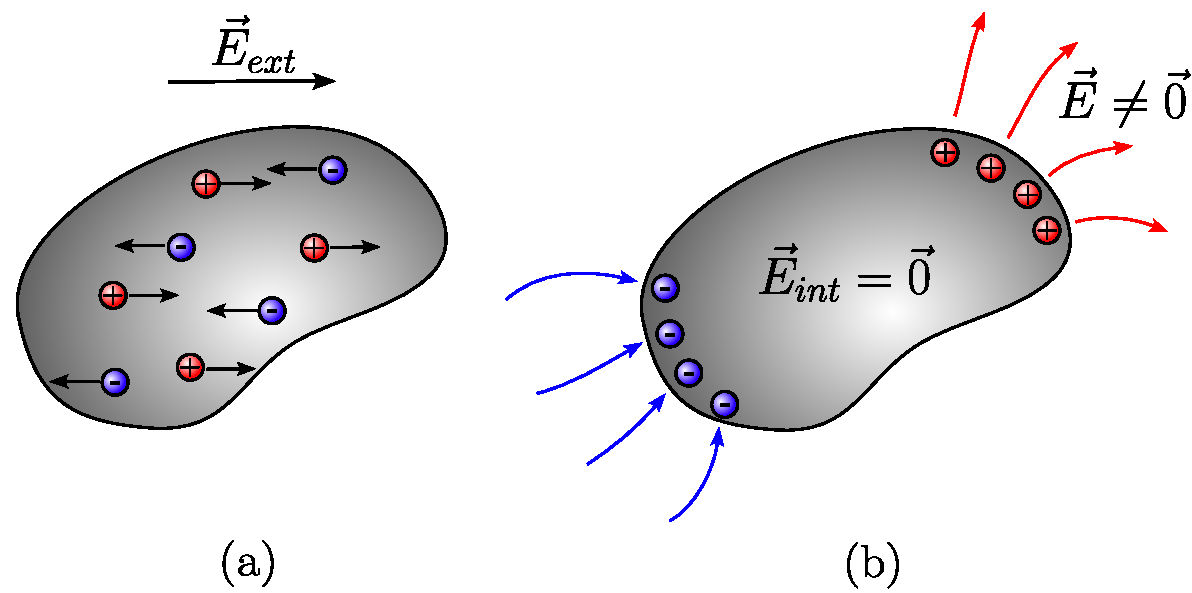
\includegraphics[scale = 0.6]{Figuras/Conductor.pdf}
    \caption{Conductor sometido a un campo externo (a) para luego entrar en equilibrio electrostático (b).}
    \label{fig:Conductor}
\end{figure}

Un conductor en equilibrio electrostático tiene las siguientes propiedades:

\begin{enumerate}
\item El campo eléctrico dentro  de un conductor en equilibrio electrostático es nulo.

\textbf{Explicación:} Para lograr el equilibrio, las cargas se distribuyen de tal manera que ellas no sufran ninguna fuerza neta. Como consecuencia $\vec{E}_{int} = \vec{0}$, pero al estar las cargas separadas (polarizadas), estas generarían un campo eléctrico que irradia hacia el exterior del conductor.

\item Cualquier carga neta en un conductor aislado debe estar en la superficie, no necesariamente de manera uniforme.

\textbf{Explicación:} Supongamos que tenemos un conductor cargado. Imaginemos una superficie gaussiana muy cercana a la superficie del conductor, ver figura \ref{fig:Gauss-Conductor}.

\begin{figure}[H]
    \centering
    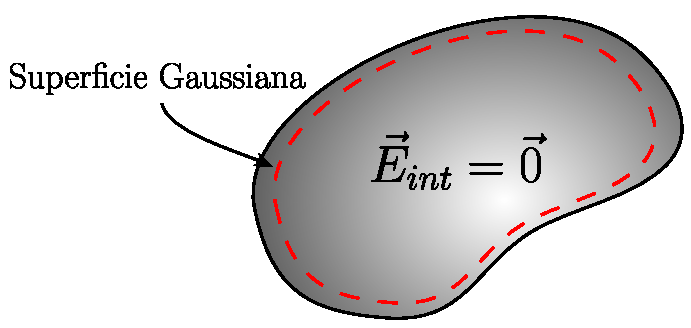
\includegraphics[scale = 0.57]{Figuras/Conductor-Gauss.pdf}
    \caption{}
    \label{fig:Gauss-Conductor}
\end{figure}

La ley de Gauss nos dice que el flujo a través de esa superficie debe ser igual a la carga encerrada:
$$\Phi_{E} = \oiint_S \vec{E} \cdot d\vec{S} = \frac{q_{enc}}{\varepsilon_0}.$$

Pero, puesto que $\vec{E} = \vec{0}$ en el interior, $\Phi_{E} = 0$, y en consecuencia $q_{enc} = 0$. Es decir no hay carga en el interior. Ahora, si colocamos la superficie gaussiana arbitrariamente muy cerca de la superficie conductora, el resultado es el mismo. Por lo tanto, si el conductor está cargado, la carga debe estar necesariamente en la superficie.

\item Si $A$ y $B$ son dos puntos arbitrarios sobre la superficie de un conductor, entonces $\Delta \Phi = \Phi(B) - \Phi(A) = 0$. Ésto implica que el campo eléctrico es perpendicular a la superficie.

\textbf{Explicación:} Si $\Delta \Phi \neq 0$, entonces $d\Phi = \vec{E} \cdot d\vec{x} \neq 0$. Por lo tanto, existiría una componente paralela a la superficie, lo que haría mover a las cargas en contradicción con la condición de equilibrio electrostático.

\item En un conductor de forma irregular, la densidad de carga es mayor donde el radio de curvatura de la superficie es menor.

\textbf{Explicación:} Si un conductor tiene exceso de cargas, éstas se repelerán y tratarán de estar lo más alejadas posible uno de los otras. En superficies planas la repulsión es mayor que si estuvieran en una región con alto grado de curvatura. En regiones con puntas las cargas sentirán menor repulsión entre sí y habrá una mayor densidad de carga en esa región.
\end{enumerate}

\begin{ejemplo}
    Una esfera maciza de radio $a$ y carga $Q$ uniformemente distribuida es blindada por una capa conductora de espesor uniforme $a$. La carga neta de la capa es nula. Calcule el potencial $\phi(r)$ en todo el espacio. Considere $\phi$ nulo infinitamente lejos de la esfera.
    \begin{figure}[H]
        \centering
        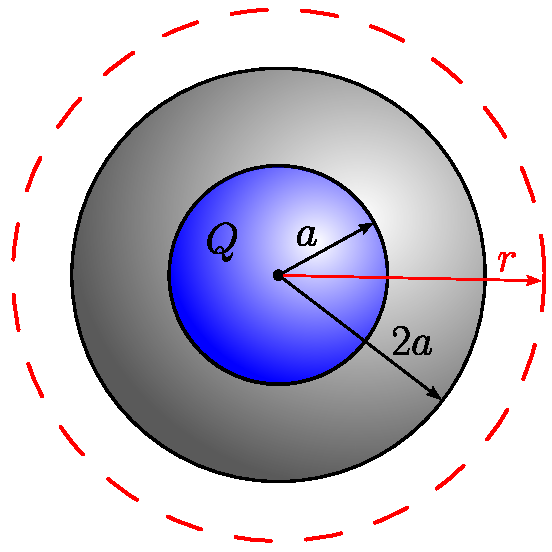
\includegraphics[scale = 0.6]{Figuras/Ej-Conductor.pdf}
        \caption{Esfera maciza de radio $a$ y carga $Q$ rodeada por una capa conductora de espesor uniforme $a$.}
        \label{fig:Ej-Conductor}
    \end{figure}
    
    \textbf{Solución:} Primero determinemos el campo eléctrico, para ello usaremos la ley de Gauss aprovechando que el campo es radial por simetría esférica. Como en ejemplos anteriores se desarrollo en detalle este tipo de cálculo, se omitirán pasos.

    Consideremos el cascarón esférico $S$ de radio $r$ centrado en el centro de la esfera maciza. 

    \begin{enumerate}
        \item Para $r > 2a$, 
        $$\oiint_S \Vec{E} \cdot d\Vec{S} = \frac{Q}{\varepsilon_0} \Rightarrow 4\pi r^2 E = \frac{Q}{\varepsilon_0} \Rightarrow \Vec{E}(r) = \frac{Q}{4\pi\varepsilon_0 r^2} \,\hat{r}.$$

        \item Para $a < r < 2a$,
        $$\Vec{E}(r) = \Vec{0}.$$

        \item Para $r< a$,
        $$\oiint_S \Vec{E} \cdot d\Vec{S} = \frac{q_{encerrada}}{\varepsilon_0} \Rightarrow 4\pi r^2 E = \frac{Q r^3}{\varepsilon_0 a^3} \Rightarrow \Vec{E}(r) = \frac{Q r}{4\pi\varepsilon_0 a^3} \,\hat{r}.$$
    \end{enumerate}

    Ahora, calculemos el potencial siguiendo una trayectoria radial desde el infinito hasta un punto con coordenada esférica $r$.

    \begin{itemize}
        \item Para $r > 2a$,
        $$\phi(r) - \phi(\infty) = -\int_{\infty}^r \Vec{E} \cdot d\vec{x} = -\int_{\infty}^r \frac{Q}{4\pi\varepsilon_0 r^2} \,dr = \frac{Q}{4\pi\varepsilon_0 r}.$$

        Si imponemos $\phi(\infty) \stackrel{!}{=} 0$, tenemos que
        $$\phi(r) = \frac{Q}{4\pi\varepsilon_0 r}.$$

        \item Para $a \leq r \leq 2 a$, tenemos que $\Vec{E}(r) = \Vec{0}$. Luego, el potencial es constante y por continuidad, tendrá el mismo valor que en la frontera $r = 2a$, es decir,
        $$\phi(r) = \phi(2a) = \frac{Q}{8\pi\varepsilon_0 a}.$$

        \item Para $r < a$, 
        \begin{align*}
            \phi(r) &= - \int_{\infty}^r E(r) \,dr \\
            &= - \left( \int_{\infty}^{2a} \frac{Q}{4\pi\varepsilon_0 r^2} \,dr + \cancelto{0}{\int_{2a}^a E(r) \,dr} + \int_a^r  \frac{Qr}{4\pi \varepsilon_0 a^3} \,dr \right) \\
            &= \frac{Q}{8\pi \varepsilon_0 a} + \frac{Q(a^2-r^2)}{8\pi \varepsilon_0 a^3}.
        \end{align*}
    \end{itemize}
\end{ejemplo}

\section{Capacitadores}

Un \textbf{capacitor} o \textbf{condensador} está formado por dos conductores aislados eléctricamente uno del otro, ya sea por medio del vacío o un aislante (dieléctrico). Uno con carga $Q$ y el otro $-Q$, ver figura \ref{fig:capacitador}.

\begin{figure}
    \centering
    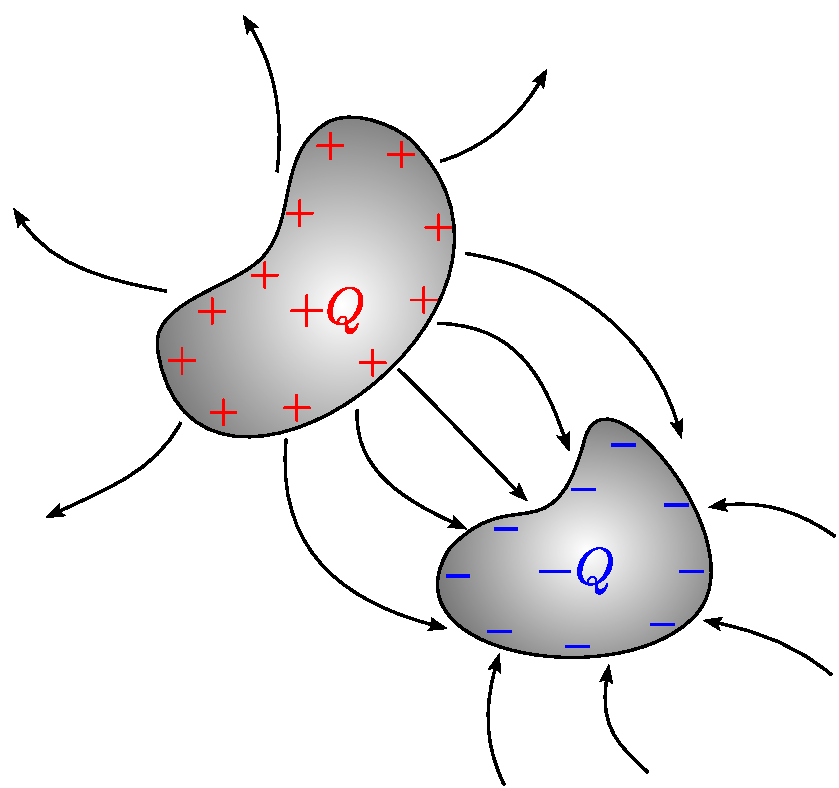
\includegraphics[scale = 0.55]{Figuras/Capacitador.pdf}
    \caption{Capacitador.}
    \label{fig:capacitador}
\end{figure}

Se puede demostrar experimentalmente que $Q \varpropto V$, y la constante de proporcionalidad $C$ se denomina \textbf{capacitancia} y se escribe como
\begin{shaded}
    $$C = \frac{Q}{|\Delta V|} = \frac{Q}{V}.$$
\end{shaded}

La unidad de medida de la capacitancia es el \textit{Faradio} ($F$) tal que
$$1 \,F  = \frac{1 \,C}{1\,V}.$$

La capacitancia de un capacitador es una propiedad física de dos conductores y depende de: la geometría del capacitor y la permitividad eléctrica $(\varepsilon)$ del medio.

\subsection*{Capacitor de placas paralelas}

Este capacitor consiste en dos placas metálicas paralelas de área $A$, cargadas con una carga $Q$ y separadas por una distancia $d$. Si ignoramos los efectos de borde podemos considerar el campo en el interior uniforme con dirección $\hat{\imath}$, es decir, estamos haciendo la aproximación de dos planos infinitos. 

\begin{figure}[H]
    \centering
    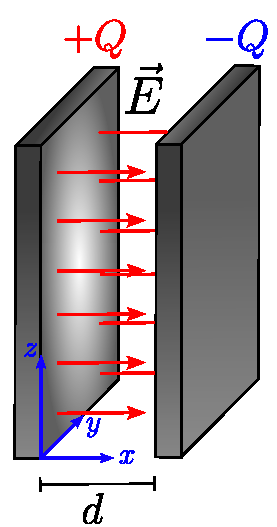
\includegraphics[scale = 0.8]{Figuras/Capacitador-Placas-Paralelas.pdf}
    \caption{Capacitador de placas paralelas.}
    \label{fig:Cap-Placas}
\end{figure}

El campo el eléctrico de un plano infinito ubicado en el plano $x = 0$, está dado por
$$\Vec{E}(x) =  \left\{ \begin{array}{cl}
   \frac{\sigma}{2 \varepsilon_0} \,\hat{\imath} ,  & \text{si} \quad x > 0  \\
    - \frac{\sigma}{2 \varepsilon_0} \,\hat{\imath}, & \text{si} \quad  x < 0 
\end{array} \right. .$$

Por consiguiente, al considerar dos planos infinitos, uno ubicado en el plano $x = 0$ y el otro en el plano $x = d$, tenemos que los campos eléctricos fuera del capacitador se cancelan, sobreviviendo solo el campo entre las placas dado por
$$\Vec{E}(x) = \frac{\sigma}{2\varepsilon_0} \,\hat{\imath} + \frac{\sigma}{2\varepsilon_0} \,\hat{\imath} = \frac{\sigma}{\varepsilon_0} \,\hat{\imath}, \quad 0 < x < d.$$

La diferencial de potencial se obtiene de
$$\Delta V = V(d) - V(0) = - \int_0^d \left(\frac{\sigma}{\varepsilon_0} \,\hat{\imath} \right) \cdot (dx\,\hat{\imath}) = - \int_0^d \frac{\sigma}{\varepsilon_0} dx = - \frac{\sigma}{\varepsilon_0} d.$$

Tomando el valor absoluto de $\Delta V$, la capacitancia es
$$C = \frac{Q}{|\Delta V|} = \frac{\sigma A}{\frac{\sigma}{\varepsilon_0} d} = \frac{\varepsilon_0 A}{d}.$$

\subsection*{Capacitador cilíndrico}

Este capacitador consiste en un cilindro sólido de radio $a$ y carga $+Q$ rodeado coaxialmente por una cáscara cilíndrica de radio $b$ y carga opuesta $-Q$. 

\begin{figure}[H]
    \centering
    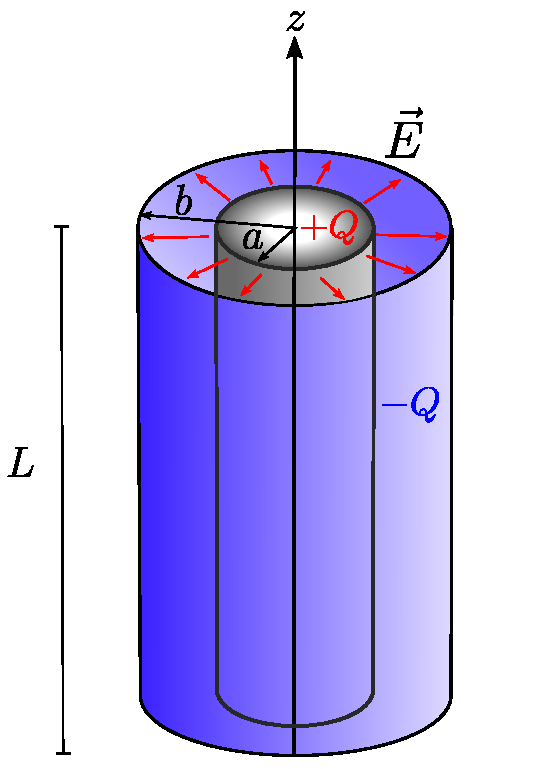
\includegraphics[scale = 0.7]{Figuras/Capacitador-Cilindrico.pdf}
    \caption{Capacitador cilíndrico.}
    \label{fig:Cap-Cilindrico}
\end{figure}

Si consideramos el largo $L$ del cilindro lo suficientemente grande, podemos aproximar el campo eléctrico al de un alambre infinito de densidad lineal de carga $\lambda$, a saber,
$$\Vec{E}(\rho) = \frac{\lambda}{2\pi \varepsilon_0 \rho}  \,\hat{\rho}, \quad a < \rho < b.$$

La diferencial de potencial entre los puntos $a$ y $b$ es
$$  \Delta V = - \int_a^b \Vec{E}(\rho) \cdot d\Vec{x}  
= - \int_a^b\frac{\lambda}{2\pi \varepsilon_0 \rho}\, d\rho 
= - \frac{\lambda}{2\pi \varepsilon_0} \int_a^b \frac{1}{\rho} \,d\rho 
= - \frac{\lambda}{2\pi \varepsilon_0} \ln\left( \frac{b}{a} \right).  $$

Entonces, la capacitancia está dada por
$$C =  \frac{Q}{|\Delta V|} = 2\pi \varepsilon_0  \frac{Q}{\lambda\ln\left(  \frac{b}{a}\right)}.$$

Pero, $\lambda = Q/L$. Por lo tanto,
$$C = 2\pi \varepsilon_0  \frac{L}{\ln\left(  \frac{b}{a}\right)}.$$

\subsection*{Capacitador esférico}

Un capacitador esférico consiste de un cascarón conductor de radio $b$ y carga $-Q$ concéntrico con una esfera conductora más pequeña de radio $a$ y carga $+Q$.

\begin{figure}[H]
    \centering
    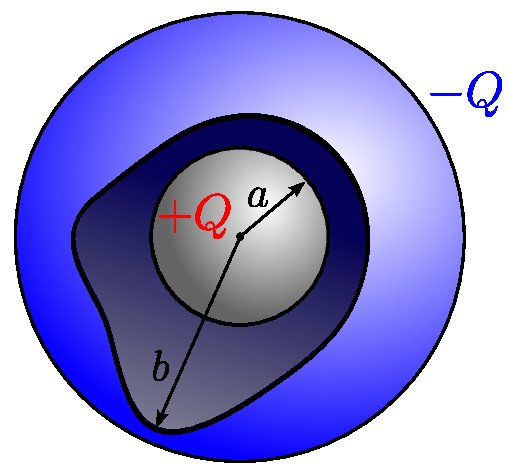
\includegraphics[scale = 0.7]{Figuras/Capacitador-Esferico.pdf}
    \caption{Capacitador esférico.}
    \label{fig:Cap-Esferico}
\end{figure}

Usando la ley de Gauss se puede encontrar fácilmente el campo eléctrico entre $a$ y $b$:
$$\Vec{E}(r) = \frac{Q}{4\pi \varepsilon_0 r^2} \,\hat{r}, \quad a < r < b.$$

La diferencial de potencial es
$$\Delta V = - \int_a^b \Vec{E}(r) \cdot d\Vec{x} = - \int_a^b \frac{Q}{4\pi \varepsilon_0 r^2} \,dr = - \frac{Q}{4\pi \varepsilon_0 r^2} \left[ - \frac{1}{r}  \right]_a^b = \frac{Q}{4\pi \varepsilon_0} \left( \frac{1}{b} - \frac{1}{a} \right).$$

Note que la diferencia de potencial es negativa. Entonces,
$$|\Delta V| = \frac{Q}{4\pi \varepsilon_0} \left( \frac{1}{a} - \frac{1}{b} \right) = \frac{Q}{4\pi \varepsilon_0} \cdot \frac{b-a}{ab}.$$

Luego, la capitancia es
$$C = \frac{Q}{|\Delta V|} = 4\pi \varepsilon_0 \frac{ab}{b-a}.$$

Note que, con la expresión anterior podemos calcular la capacitancia de un conductor aislado. Si hacemos $b \to  \infty$, la capacitancia queda
\begin{equation*}
C = \lim_{b \to \infty} \left[ 4\pi \varepsilon_0 \frac{ab}{b-a} \right] = 4\pi \varepsilon_0 \lim_{b \to \infty} \left[\frac{a}{1 - \frac{a}{b}} \right] = 4\pi \varepsilon_0 a.
\end{equation*}

\subsection*{Combinaciones de capacitadores}

\begin{enumerate}
\item \textbf{Capacitadores en serie}: En este caso dos o más capacitadores se conectan uno a continuación del otro y se supone que la fuente voltaica se ha aplicado en los extremos de esta combinación. De ello resulta que la carga de ellos es la misma. Nos interesa encontrar la capacitancia total o equivalente, es decir, el valor de la capacitancia de un solo capacitador que podría sustituir a todos los capacitadores del circuito para simplificarlo tal que el circuito resultante sea equivalente al original.

Por simplicidad, consideremos dos capacitadores cualesquiera de capacitancias $C_1$ y $C_2$ con voltajes $V_1$ y $V_2$, respectivamente.

\begin{figure}[H]
    \centering
    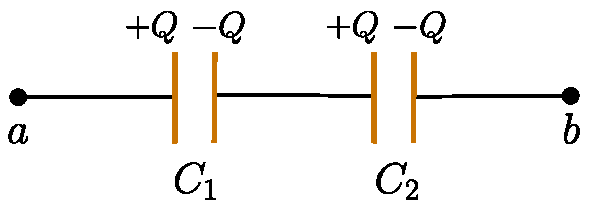
\includegraphics[scale = 0.8]{Figuras/Capacitador-Serie.pdf}
    \caption{Capacitadores en serie.}
    \label{fig:Cap-Serie}
\end{figure}

De la definición de capacitancia:
$$C_1 = \frac{Q}{V_1} ~~\text{y}~~ C_2 = \frac{Q}{V_2}.$$

Pero $V_1 + V_2 = V_{ab}$. Luego,
$$V_{ab} = V_1 + V_2 = \frac{Q}{C_1} + \frac{Q}{C_2}.$$

Entonces, la capacitancia equivalente a la combinación es
\begin{align*}
  V_{ab} = V_1 + V_2 
&\Rightarrow  \frac{Q}{C_{eq}} = \frac{Q}{C_1} + \frac{Q}{C_2} \\
&\Rightarrow  \frac{1}{C_{eq}} = \frac{1}{C_1} + \frac{1}{C_2}.  
\end{align*}

Generalizando para $n$ capacitadores en serie:
\begin{shaded}
    $$\frac{1}{C_{eq}} = \sum_{i=1}^n \frac{1}{C_i}$$
\end{shaded}

\item \textbf{Capacitadores en paralelo}: En este caso se unen entre si los extremos de los capacitadores a un lado de ellos y los otros extremos también se unen entre si, ver figura \ref{fig:Cap-Paralelo}. De ello resulta que todos tienen la misma diferencial de potencial.

\begin{figure}[H]
    \centering
    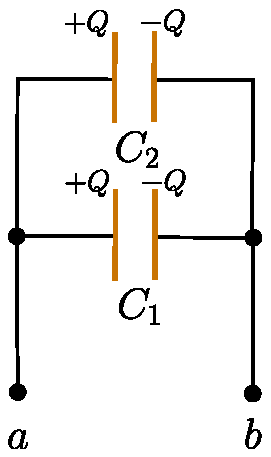
\includegraphics[scale = 0.8]{Figuras/Capacitador-Paralelo.pdf}
    \caption{Capacitadores en paralelo.}
    \label{fig:Cap-Paralelo}
\end{figure}

De la definición de capacitancia:
$$C_1 = \frac{Q}{V_1} ~~\text{y}~~ C_2 = \frac{Q}{V_2}.$$

Como $V_1 = V_2 = V_{ab}$, se tiene que
$$Q_1 = C_1 V_{ab}  ~~\text{y}~~ Q_2 = C_2 V_{ab}.$$

La carga producida se distribuye, es decir, $Q= Q_1 + Q_2$ con $Q = V_{ab} C_{eq}$, entonces
$$V_{ab}C_{eq} = V_{ab} C_1 +  V_{ab} C_2 \Rightarrow C_{eq} = C_1 + C_2.$$

Generalizando para $n$ capacitadores en paralelo:
\begin{shaded}
    $$C_{eq} = \sum_{i=1}^n C_i.$$
\end{shaded}

\end{enumerate}

\subsection*{Energía de un capacitador en el vacío}

Para hacer este cálculo supondremos que  un agente externo lleva elementos de carga $dq$ desde el lado de menor potencial al de potencial mayor (de la placa negativa a la positiva), ésto es, contra del potencial. Consideremos un instante en que la carga del lado positivo es $q$ y que el voltaje entre ambos elementos del capacitador es $V$, dado que el trabajo elemental hecho por la fuerza externa equilibrante es igual al incremento de energía potencial, se tiene que
$$dU = V \,dq = \frac{q}{C} \,dq.$$

Si durante este proceso se transfiere una carga $Q$ de una placa a otra:
$$U = \int_0^Q \frac{q}{C} \,dq = \frac{Q^2}{2C}.$$

Usando $Q = CV$ queda
\begin{shaded}
 \begin{equation*}
U = \frac{1}{2} CV^2
\end{equation*}
\begin{center}
(Energía almacenada en el capacitador)
\end{center}   
\end{shaded}

\subsection*{Densidad de energía eléctrica}

La \textbf{densidad de energía} es la energía  almacenada en un campo eléctrico por unidad de volumen, es decir,
$$u := \frac{dU}{dv}.$$

Si la energía es uniforme, entonces $u = U/v$.

En el caso del campo de un condensador plano:
$$u = \frac{U}{v} = \frac{\frac{1}{2}CV^2}{Ad} = \frac{\frac{1}{2} \left( \frac{\varepsilon_0 A}{d} \right)V^2}{Ad} = \frac{1}{2} \varepsilon_0 \left( \frac{V}{d} \right)^2.$$

Como $V = Ed$,
\begin{shaded}
   $$ u = \frac{1}{2} \varepsilon_0 E^2.$$
\end{shaded}

Este resultado, obtenido para un capacitador plano, se puede generalizar al campo de otros capacitadores, incluso para una esfera.

\begin{ejemplo}
Cosidere una esfera con carga total $Q$ y radio $R$. Si la carga se encuentra distribuida uniformemente, calcule la energía almacenada en la intensidad del campo electrostático generado por la distribución esférica.

\textbf{Solución:} Recordemos que el campo electrostático de una esfera de densidad de carga uniforme de radio $R$, en coordenadas esféricas, está dado por
$$\Vec{E}(r) =  \left\{ \begin{array}{cl}
   \frac{Q}{4\pi \varepsilon_0 r^2} \,\hat{r}  ,  & \text{si} \quad r \geq R  \\
    \frac{Qr}{4\pi \varepsilon_0 R^3}\,\hat{r}, & \text{si} \quad  0 < r < R 
\end{array} \right. .$$

De la definición de densidad de energía:
$$u = \frac{d U}{dv} = \frac{1}{2} \varepsilon_0 E^2 \Rightarrow dU = \frac{1}{2} \varepsilon_0 E^2 dv.$$

Integrando en todo el espacio, usando coordenadas esféricas, se tiene que
\begin{align*}
U &= \int_0^{\infty} \int_0^{\pi} \int_0^{2\pi} \frac{1}{2} \varepsilon_0 E^2 r^2 \sin\theta \,d\varphi \,d\theta \,dr \\
&= \frac{1}{2} \varepsilon_0 \left\{ \int_0^R \int_0^{\pi} \int_0^{2\pi} \frac{Q^2r^2}{16\pi^2 \varepsilon_0^2 R^6} r^2 \sin\theta \,d\varphi\, d\theta \,dr + \int_R^{\infty} \int_0^{\pi} \int_0^{2\pi} \frac{Q^2}{16\pi^2 \varepsilon_0^2 r^4} r^2 \sin\theta \,d\varphi \,d\theta \,dr \right\} \\
&= \frac{Q^2 }{32\pi^2 \varepsilon_0} \left\{ \frac{1}{R^6}\int_0^R r^4 \int_0^{\pi} \sin\theta \int_0^{2\pi} d\varphi \,d\theta \,dr + \int_R^{ \infty} \frac{1}{r^2} \int_0^{\pi} \sin \theta \int_0^{2\pi} d\varphi \,d\theta \,dr \right\} \\
&= \frac{2\pi Q^2}{32 \pi^2 \varepsilon_0} \left\{ \frac{1}{R^6} \int_0^R r^4 \int_0^{\pi} \sin \theta \,d\theta \,dr + \int_R^{\infty} \frac{1}{r^2} \int_0^{\pi} \sin\theta \,d\theta\, dr\right\} \\
&= \frac{2Q^2}{16 \pi \varepsilon_0} \left\{ \frac{1}{R^6} \int_0^R r^4 \,dr + \int_R^{\infty} \frac{1}{r^2} \,dr \right\} \\
&= \frac{Q^2}{8 \pi \varepsilon_0} \left\{ \frac{1}{R^6} \left[ \frac{r^5}{5} \right]_0^R + \left[ - \frac{1}{r} \right]_R^{\infty} \right\} \\
&= \frac{Q^2}{8\pi \varepsilon_0} \left\{ \frac{1}{5R} + \frac{1}{R} \right\} \\
&= \frac{3Q^2}{20\pi \varepsilon_0 R}.
\end{align*}
\end{ejemplo}

\section{Campo eléctrico en la materia}

\subsection{Dieléctricos}

Un material \textbf{dieléctrico} es un aislante que al ser sometido a un campo eléctrico externo ($\vec{E}_0$), éste se poraliza. En otras palabras, se producen desplazamientos de cargas dentro de las moléculas de tal forma que se crean pequeños \underline{dipolos eléctricos}.

\begin{figure}[H]
    \centering
    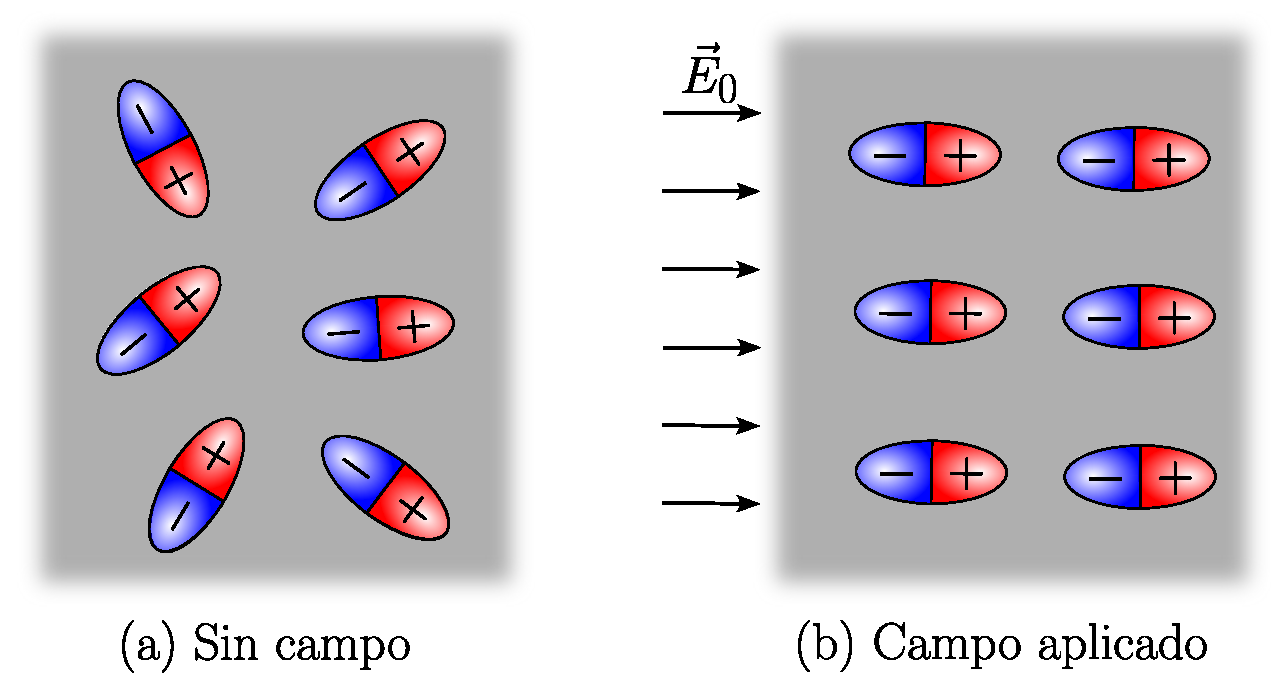
\includegraphics[scale = 0.5]{Figuras/Dielectrico.pdf}
    \caption{Orientación de los dipolos de un dieléctrico en presencia de un campo eléctrico externo.}
    \label{fig:Dielectrico}
\end{figure}

Las cargas de polarización (dipolos) crean un campo eléctrico en dirección contraria al externo, llamado \textbf{campo de polarización}, $\vec{E}_p$, de manera que el campo total es:
$$\vec{E} = \vec{E}_0 + \vec{E}_p.$$

O en forma escalar 
\begin{equation}
E = E_0 - E_p. \label{CampoTotal}
\end{equation}

El dieléctrico tiene el efecto de disminuir el campo externo y depende del dieléctrico elegido.

Note que con solo la ecuación \eqref{CampoTotal}, no podemos saber el campo total en un dieléctrico, pues hay dos incógnitas ($E$, $E_p$). Aquí, entra la Física proponiendo el siguiente modelo:
$$\vec{E}_p = - \chi \vec{E},$$

donde $\chi$ es definida como una cantidad positiva llamada \textbf{susceptibilidad eléctrica}.

Luego,
$$\vec{E} = \vec{E}_0 - \chi \vec{E} \Rightarrow  (1+\chi)\vec{E} = \vec{E}_0 \Rightarrow  \vec{E} = \frac{\vec{E}_0}{1+\chi}.$$

Se define la \textbf{constante dieléctrica} $\kappa > 1$ como
\begin{shaded}
$$\kappa := 1 + \chi,$$    
\end{shaded}

quedando
\begin{shaded}
  $$\vec{E} = \frac{\vec{E}_0}{\kappa}.$$  
\end{shaded}

A continuación, una tabla con algunas constantes dieléctricas con su respectivo campo de ruptura dieléctrica que simbolizamos con $E_M$. Éste es el máximo campo que soporta el dieléctrico antes de que salte en él una chispa por ionización.

\begin{center}
\begin{tabular}{|c|c|c|}
\hline 
Material & $\kappa$ & $E_M (10^6 \,[V/m])$ \\
\hline 
Vacío & 1.00000 & $\infty$ \\
Aire seco &  1.0006 & 3 \\
Agua & 78 & --- \\
Papel seco & 3.7 & 16 \\
Vidrio & 5.6 & 14 \\
\hline
\end{tabular}
\end{center}

\subsubsection{Capacitador lleno con dieléctrico}

Podemos encontrar fácilmente la relación entre la capacitancia de un capacitador lleno con dieléctrico, de cualquier forma geométrica, con la de uno vacío.

\begin{itemize}
\item[i)] \textbf{Sin dieléctrico}: El capacitador ha sido cargado con voltaje $V_0$ y ha adquirido una carga libre $Q_0$, y después se ha desconectado de la fuente voltaica.

\begin{figure}[H]
    \centering
    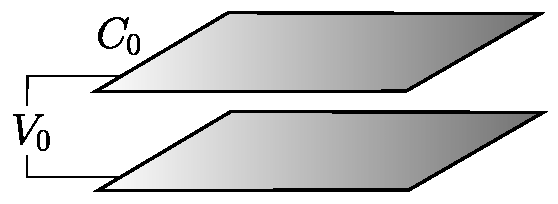
\includegraphics[scale = 0.6]{Figuras/Capacitador-Sin-Dielectric.pdf}
    \caption{Capacitador sin dieléctrico.}
    \label{fig:Cap-Sin-Dielectrico}
\end{figure}

La capacidad está dada por
$$C_0 = \frac{Q_0}{V_0} ~~\mbox{en que}~~ V_0 = \int \vec{E}_0 \cdot d\vec{x}.$$

\item[ii)] \textbf{Con dieléctrico}: El mismo capacitador se ha llenado con dieléctrico y al estar desconectado conserva su carga $Q_0$.

\begin{figure}[H]
    \centering
    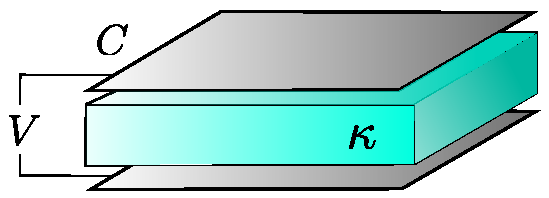
\includegraphics[scale = 0.6]{Figuras/Capacitador-ConDielectrico.pdf}
    \caption{Capacitador con dieléctrico.}
    \label{fig:Cap-Con-Dielectrico}
\end{figure}

 En este caso,
$$C = \frac{Q_0}{V},$$

donde 
$$V = \int \vec{E} \cdot d\vec{x} = \frac{1}{\kappa}\int \vec{E}_0 \cdot d\vec{x} = \frac{V_0}{\kappa}. $$

Luego,
\begin{shaded}
 $$C = \frac{Q_0}{V_0 / \kappa} = \kappa C_0,$$   
\end{shaded}

es decir, la nueva capacitancia aumentó en un factor $\kappa$. 

Puesto que su voltaje disminuyó, entonces puede adquirir más carga si se aplica de nuevo la fuente. En ese caso,
\begin{equation*}
C = \frac{Q}{V_0} = \kappa C_0 ~~\mbox{y}~~ Q = \kappa C_0 V_0 = \kappa Q_0.
\end{equation*}

\end{itemize}

\begin{ejemplo}
   Calcular la capacitancia de un capacitador plano, de área $A$, separación $d$ y lleno con tres dieléctricos de espesor $d_1$, $d_2$ y $d_3$, y constantes dieléctricas $\kappa_1$, $\kappa_2$ y $\kappa_3$, respectivamente.

\begin{figure}[H]
    \centering
    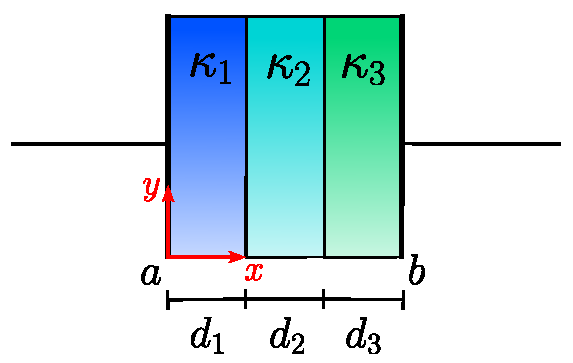
\includegraphics[scale = 0.7]{Figuras/Ej-Dielectrico.pdf}
    \caption{Capacitador lleno de tres dieléctricos.}
    \label{fig:Ej-Dielectrico}
\end{figure}

\textbf{Solución:} Por definición del potencial electrostático,
\begingroup
\allowdisplaybreaks
\begin{align*}
    V_{ab} = V(a) - V(b) &= \int_0^d \Vec{E} \cdot d\Vec{x} \\
    &= \int_0^d (E \,\hat{\imath}) \cdot (dx\, \hat{\imath}) \\
&= \int_0^d E \,dx \\
&= \int_0^{d_1} \frac{E_0}{\kappa_1} \,dx + \int_{d_1}^{d_1 + d_2} \frac{E_0}{\kappa_2} \,dx + \int_{d_1 + d_2}^{d_1  + d_2 + d_3} \frac{E_0}{\kappa_3} \,dx  \\
&= \frac{E_0}{\kappa_1} d_1 + \frac{E_0}{\kappa_2} d_2 + \frac{E_0}{\kappa_3} d_3.
\end{align*}
\endgroup

Luego, la capacitancia está dada por
$$C = \frac{Q}{V_{ab}} = \frac{Q_0}{\frac{E_0}{\kappa_1} d_1 + \frac{E_0}{\kappa_2} d_2 + \frac{E_0}{\kappa_3} d_3}.$$

Recordando que para un capacitador de placas paralelas: $E_0 = \frac{\sigma_0}{\varepsilon_0}$ y que $Q_0 = \sigma A$. Por lo tanto,
\begin{align*}
    C &= \frac{\sigma_0 A}{\frac{\sigma_0}{\varepsilon_0 \kappa_1} d_1 + \frac{\sigma_0}{\varepsilon_0 \kappa_2} d_2 + \frac{\sigma_0}{\varepsilon_0  \kappa_3} d_3} \\ 
    &= \frac{\varepsilon_0 A}{\frac{d_1}{\kappa_1} + \frac{d_2}{\kappa_2}  + \frac{d_3}{\kappa_3}}.
\end{align*}
  
\end{ejemplo}

\subsubsection{Energía de capacitadores con dieléctrico}

La relación para la energía o de la densidad de energía se mantienen cambiando $\varepsilon_0$ por $\varepsilon = \kappa \varepsilon_0$, ya que las consideraciones físicas en su deducción no cambian.

Así, para un capacitador plano lleno de un dieléctrico vemos que la capacitancia está dada por
$$C = \kappa C_0 = \kappa \varepsilon_0 \frac{A}{d} = \varepsilon \frac{A}{d}.$$

Su energía es
\begin{shaded}
    $$U = \frac{1}{2} C V^2 = \kappa U_0.$$
\end{shaded}

La densidad de energía de un medio dieléctrico es
\begin{shaded}
    $$u = \frac{1}{2} \varepsilon E^2.$$
\end{shaded}

\subsubsection{Densidad de polarización}

La aparición de $\Vec{E}_{p}$ en el capacitor de placas paralelas es equivalente a la aparición de una densidad de carga superficial en ambas caras del dieléctrico, ver figura \ref{fig:densidad-polarizacion}.

\begin{figure}[H]
    \centering
    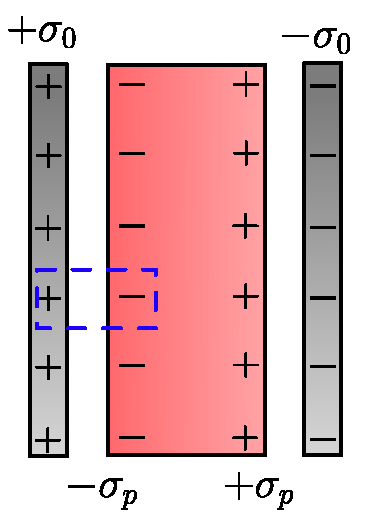
\includegraphics[scale = 0.7]{Figuras/Densidad-Polarizacion.pdf}
    \caption{Densidad de polarización}
    \label{fig:densidad-polarizacion}
\end{figure}

Usando la ley de Gauss al cilindro de radio $R$ que tiene una tapa en el dieléctrico y la otra tapa dentro del conductor tal que el campo eléctrico sea nulo,
\begin{align*}
    \oiint_S \Vec{E} \cdot d\Vec{S} &= \frac{q_{enc}}{\varepsilon_0} \\
    \int_{S_{tapa}} \Vec{E} \cdot d\Vec{S} &= \frac{1}{\varepsilon_0}\int_0^R \int_0^{2\pi} (\sigma_0 - \sigma_p) \rho\,d\varphi\,d\rho \\
    \int_0^R \int_0^{2 \pi} (E\,\hat{k}) \cdot (\rho \,d\varphi \,d\rho \,\hat{k}) &= \frac{2\pi (\sigma_0 - \sigma_p)}{\varepsilon_0} \int_0^R \rho \,d\rho \\
    \pi R^2 E &= \frac{\pi R^2(\sigma_0 - \sigma_p)}{\varepsilon_0} \\
    E&= \frac{\sigma_0 - \sigma_p}{\varepsilon_0}.
\end{align*}

Pero $E =  \frac{E_0}{\kappa} = \frac{\sigma_0}{\kappa \varepsilon_0}$, entonces igualando 
\begin{shaded}
 \begin{equation}
\sigma_p = \sigma_0 \left(  1- \frac{1}{\kappa} \right) \label{densidadDePolarizacion}
\end{equation}
\end{shaded}

Multiplicando por el área del capacitador, encontramos que la carga de polarización es
\begin{shaded}
    $$q_p = q_0 \left(  1- \frac{1}{\kappa} \right).$$
\end{shaded}

\subsection{Vector de polarización*}

Formalicemos la discusión hecha para materiales dieléctricos. Al estar en presencia de un campo externo, si el dieléctrico esta formado por átomos neutros (o moléculas apolares), el campo inducirá en cada uno un pequeño momento dipolar, apuntando en la misma dirección del campo. Si el dieléctrico está hecho de moléculas polares, cada dipolo permanente experimentará un torque, tendiendo a alinearse en la dirección del campo. 

En los dos casos discutidos se tiene el mismo resultado: varios ``dipolitos'' apuntando en la dirección del campo. El material se dice que se \textit{polariza}. Para medir este efecto definimos al  \textbf{vector de polarización} $\Vec{P}$ como la densidad de momento dipolar,
$$\Vec{P}(\Vec{x}) := ``\lim_{\Delta V \to 0}" \frac{\sum \Vec{p}_i}{\Delta V},$$

donde $\sum\Vec{p}_i$ es el \textit{momento dipolar total de las cargas del material contenidas en el volumen $\Delta V$}. La región con volumen $\Delta V$ se considera centrada en el punto $\Vec{x}$, suficientemente pequeña desde el punto de vista macroscópico, pero grande comparada con la escala determinada por la estructura atómica/molecular del material. 

 \begin{figure}[H]
     \centering
     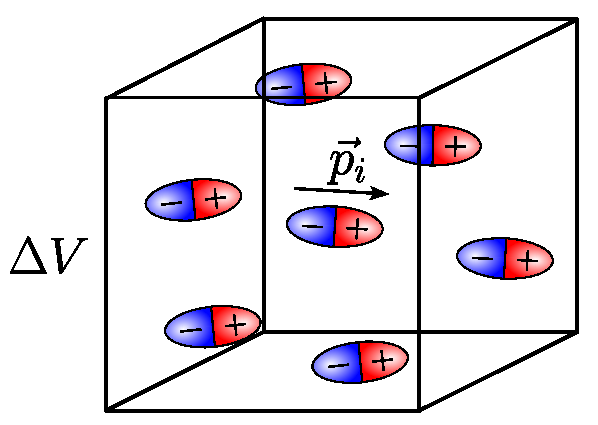
\includegraphics[scale = 0.6]{Figuras/Polarizacion.pdf}
     \caption{Dipolos en un volumen $\Delta V$.}
     \label{fig:Polarizacion-Volumen}
 \end{figure}

Equivalentemente, el vector de polarización es definido tal que el momento dipolar $d\Vec{p}$ en un elemento de volumen (macroscópico) $dV$ es dado por $d\Vec{p} = \Vec{P}(\Vec{x})\,dV$ \footnote{De forma análoga a la densidad de carga.}. En consecuencia, el momento dipolar total de las cargas contenidas en un volumen $V$ está dado por
$$\Vec{p}_V = \iiint_V \Vec{P}(\Vec{x}) \,dV.$$ 

De la ecuación \eqref{Potencial-Dipolo-Ideal}, tenemos que el potencial generado por un dipolo ideal de momento dipolar $\Vec{p}$ ubicado en el origen es 
$$\phi_{dip}(\Vec{x}) = \frac{1}{4\pi \varepsilon_0} \frac{\Vec{p} \cdot \hat{r}}{r^2} = \frac{1}{4\pi \varepsilon_0} \frac{\Vec{p} \cdot \Vec{x}}{|\Vec{x}|^3},\quad \Vec{x} = r\,\hat{r}.$$

Ahora, si el dipolo se ubica en $\Vec{x}\,'$, efectuamos una traslación de tal forma que el potencial nos queda
$$\phi_{dip}(\Vec{x}) = \frac{1}{4\pi \varepsilon_0} \frac{\Vec{p} \cdot (\Vec{x} - \Vec{x}\,')}{|\Vec{x} - \Vec{x}\,'|^3}.$$

Luego, el potencial generado por una pequeña región de un medio polarizado con elemento de volumen $dV'$ y polarización $\Vec{P}$ es dada por

\begin{figure}[H]
    \centering
    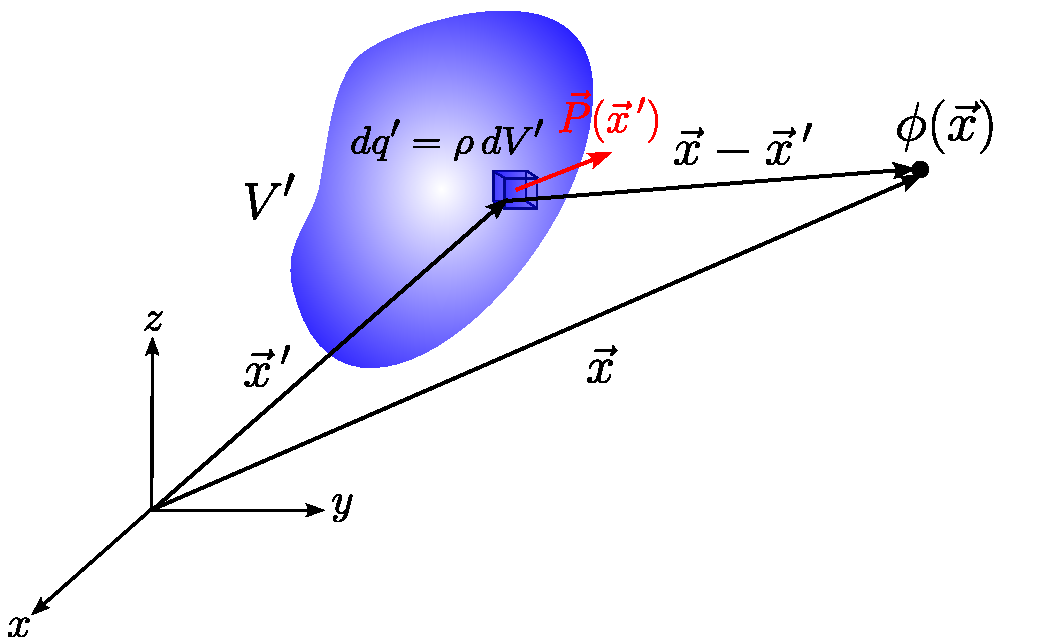
\includegraphics[scale = 0.6]{Figuras/Distribucion-Cargas-Polarizacion.pdf}
    \caption{Distribución de carga.}
    \label{fig:Distribu-Carga-3}
\end{figure}

$$d\phi(\Vec{x}) = \frac{1}{4\pi\varepsilon_0} \frac{\Vec{P}(\Vec{x}\,') \cdot (\Vec{x} - \Vec{x}\,') \,dV'}{|\Vec{x} - \Vec{x}\,'|^3}.$$

Por lo tanto, el potencial (macroscópico), bajo el modelo de considerar el dieléctrico como una ``nube" de dipolos ideales, está dado por 
\begin{shaded}
    $$\phi(\Vec{x}) = \frac{1}{4\pi \varepsilon_0} \iiint_V \frac{\Vec{P}(\Vec{x}\,') \cdot (\Vec{x} - \Vec{x}\,') }{|\Vec{x} - \Vec{x}\,'|^3} \,dV'$$
\end{shaded}

Usando la identidad \eqref{Identidad-Grad}, podemos escribir
\begin{align*}
    \frac{\Vec{P}(\Vec{x}\,') \cdot (\Vec{x} - \Vec{x}\,')}{|\Vec{x} - \vec{x}\,'|^3} &= \Vec{P}(\Vec{x}\,') \cdot \Vec{\nabla}\,' \left( \frac{1}{|\Vec{x} - \Vec{x}\,'|^3} \right) \\
    &= \Vec{\nabla}\,' \cdot \left( \frac{\Vec{P}(\vec{x}\,')}{|\Vec{x} - \Vec{x}\,'|} \right) - \frac{\Vec{\nabla}\,' \cdot \Vec{P}(\Vec{x}\,')}{|\Vec{x} - \Vec{x}\,'|},
\end{align*}

donde $\Vec{\nabla}\,'$ es el operador nabla con las derivadas parciales con respecto a las coordenadas primas $(x',y',z')$ en el dieléctrico.  

Sea $S'$ la superficie que encierra al volumen $V'$ con elemento de superficie $d\Vec{S}' = \hat{n} dS'$, por el teorema de Gauss,
\begin{align*}
    \phi(\Vec{x}) &= \frac{1}{4\pi\varepsilon_0} \left[ \iiint_{V'} \Vec{\nabla}\,' \cdot \left( \frac{\Vec{P}(\vec{x}\,')}{|\Vec{x} - \Vec{x}\,'|} \right) \,dV' -  \iiint_{V'} \frac{\Vec{\nabla}\,' \cdot \Vec{P}(\Vec{x}\,')}{|\Vec{x} - \Vec{x}\,'|} \,dV'\right] \\
    &= \frac{1}{4\pi \varepsilon_0} \iint_{S'}  \frac{\Vec{P}(\vec{x}\,') \cdot \hat{n}}{|\Vec{x} - \Vec{x}\,'|} \,dS' - \frac{1}{4\pi \varepsilon_0} \iiint_{V'} \frac{\Vec{\nabla}\,' \cdot \Vec{P}(\Vec{x}\,')}{|\Vec{x} - \Vec{x}\,'|} \,dV'.
\end{align*}

El primer término se ve como el potencial de una superficie cargada con densidad de carga
\begin{shaded}
    $$\sigma_p := \vec{P} \cdot \hat{n},$$
\end{shaded}

mientras que el segundo término se ve como el potencial de un volumen con densidad de carga
\begin{shaded}
    $$\rho_p := - \Vec{\nabla} \cdot \Vec{P}.$$
\end{shaded}

Así, el potencial total es 
\begin{shaded}
    $$\phi(\Vec{x}) = \frac{1}{4\pi \varepsilon_0} \iint_{S'}  \frac{\sigma_p(\vec{x}\,')}{|\Vec{x} - \Vec{x}\,'|} \,dS' + \frac{1}{4\pi \varepsilon_0} \iiint_{V'} \frac{\rho_p(\Vec{x}\,')}{|\Vec{x} - \Vec{x}\,'|} \,dV'.$$
\end{shaded}


\textbf{Observación:} Note que la carga total de polarización, tal como se espera, es nula:
$$Q_p = \iiint_V \rho_p \,dV + \oiint_{S} \sigma_p \,dS = \iiint_V \Vec{\nabla} \cdot \Vec{P} \,dV - \iiint_{V} \Vec{\nabla} \cdot \Vec{P}  \,dV = 0,$$

donde se usó el teorema de Gauss.

\begin{ejemplo}
    Considere una esfera de radio $R$ polarizada radialmente con
    $$\Vec{P} = P_0 \,\hat{r},$$

    donde $P_0$ es una constante.
    \begin{itemize}
        \item[(a)] Calcule las densidades de polarización $\sigma_p$ y $\rho_p$.

        \item[(b)] Encuentre el campo eléctrico en el interior y exterior de la esfera.
    \end{itemize}
    
    \textbf{Solución:} En el interior de la esfera, 
    $$\rho_p = - \Vec{\nabla} \cdot \Vec{P} = - \frac{1}{r^2} \frac{d}{dr}(r^2 P_0) = - \frac{2P_0}{r}, \quad r < R,$$

    y nulo en el exterior. La densidad superficial de carga es
    $$\sigma_p = \Vec{P} \cdot \hat{n} = ( P_0 \,\hat{r}) \cdot \hat{r} = P_0.$$

     \begin{figure}[H]
        \centering
        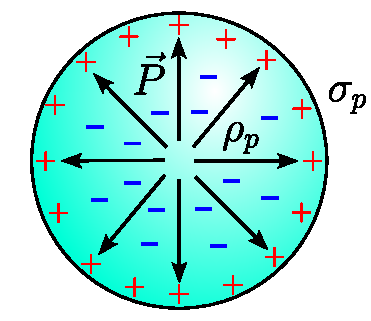
\includegraphics[scale = 0.65]{Figuras/Ej-Polarizacion.pdf}
        \caption{Esfera polarizada radialmente.}
        \label{fig:Esfera-Polarizada-Radial}
    \end{figure}

    Ahora calculemos el campo eléctrico, para ello determinaremos el campo eléctrico de una distribución de carga con 
    $$\rho_p = \left\{\begin{array}{cl}
        -\frac{2P_0}{r}, & \mbox{si} ~ r < R  \\
        0, & \mbox{si} ~ r > R  
    \end{array} \right., \quad \sigma_p = P_0 \quad (r = R),$$

    y nos aprovecharemos de que la distribución posee simetría esférica.

    Luego podemos suponer que el potencial eléctrico sólo depende de la coordenada $r$: $\phi = \phi(r)$ y, en consecuencia, el campo eléctrico es radial, pues
    $$\Vec{E} = - \Vec{\nabla} \phi = - \frac{d \phi}{dr} \,\hat{r} = E(r) \,\hat{r}.$$

    Usando la ley de Gauss a una superficie $S$ esférica de radio $r$ concéntrica con la esfera dieléctrica, el flujo del campo eléctrico es
    $$\oiint_S \Vec{E} \cdot d\Vec{S} = \iint E(r) \,dS = 4\pi r^2 E.$$

    \begin{itemize}
        \item Si $r < R$, por la ley de Gauss,
        $$4\pi r^2 E = \frac{q_{enc}}{\varepsilon_0} = \frac{1}{ \varepsilon_0} \iiint_{r < R} \rho_p \,dV.$$

        La carga encerrada es
        \begin{align*}
            q_{enc} = \iiint_{r < R} \rho_p \,dV &= \int_0^r \int_0^{\pi} \int_0^{2\pi} \left( - \frac{2P_0}{r'}\right) r'\,^2 \sin \theta \,d\varphi \,d\theta \,dr' \\
            &= - 8\pi P_0 \int_0^r r' \,dr' \\
            &= - 4\pi P_0 r^2
        \end{align*}

        y el campo eléctrico está dado por
        $$4\pi r^2 E = - \frac{4\pi P_0 r^2}{\varepsilon_0} \Rightarrow \Vec{E} = - \frac{P_0}{\varepsilon_0} \, \hat{r} = - \frac{\Vec{P}}{\varepsilon_0}.$$

        \item Si $r > R$, debemos tener en consideración la carga en el volumen como en la superficie, la cual es nula por lo demostrado. Entonces,
        $$\Vec{E} = \Vec{0}, \quad r  > R.$$
    \end{itemize}

    Combinando ambos resultados,
    $$\Vec{E} = \left\{\begin{array}{cl}
        -\frac{\Vec{P}}{\varepsilon_0}, & \mbox{si} ~ r < R  \\
        0, & \mbox{si} ~ r > R  
    \end{array} \right..$$
\end{ejemplo}

\subsection{Vector de desplazamiento*}

Vimos que cuando un dieléctrico está polarizado, aparece una densidad volumétrica de carga $\rho_p$. Esta densidad genera a su vez un campo eléctrico, el cual se superpone a cualquier otro campo eléctrico presente. Este campo es generado por, lo que llamaremos, \textbf{cargas libres} (o \textbf{externas}), con densidad de carga $\rho_{libre}$. Entonces, dentro del dieléctrico, la densidad de carga puede ser escrita como:
$$\rho =  \rho_{libre} + \rho_p,$$

y usando la forma diferencial de la ley de Gauss, tenemos que el campo eléctrico total (no solo el generado por la polarización) verifica que 
$$\Vec{\nabla} \cdot \Vec{E} = \frac{1}{\varepsilon_0} (  \rho_{libre} + \rho_p).$$


Pero, $\rho_{p} = - \Vec{\nabla} \cdot \Vec{P}$. Luego,
$$\Vec{\nabla} \cdot \Vec{E} = \frac{1}{\varepsilon_0} (\rho - \Vec{\nabla} \cdot \vec{P}).$$

Reordenando,
$$\Vec{\nabla} \cdot ( \varepsilon_0 \Vec{E} + \Vec{P}) = \rho_{libre}.$$

La expresión entre paréntesis se conoce como el \textbf{vector de desplazamiento eléctrico},
\begin{shaded}
    $$\Vec{D} := \varepsilon_0 \Vec{E} + \Vec{P}.$$
\end{shaded}

Por lo tanto, en términos de $\Vec{D}$, la forma diferencial de la ley de Gauss se puede escribir, de forma más general, como
\begin{shaded}
    $$\Vec{\nabla} \cdot \Vec{D} = \rho_{libre}.$$
\end{shaded}

Usando el teorema de Gauss, es directo probar la forma integral,
\begin{shaded}
    $$\oiint_S \Vec{D} \cdot d\Vec{S} = q_{libre},$$
\end{shaded}

donde $q_{libre}$ denota la carga total libre encerrada en el volumen.

\subsection{Susceptibilidad eléctrica y constante dieléctrica*}

El grado de polarización de un dieléctrico va a depender de la naturaleza molecular del dieléctrico y también del campo eléctrico aplicado. A nivel macroscópico, experimentalmente se ha encontrado que $\Vec{P}$ depende de $\Vec{E}$, $\Vec{P} = \Vec{P}(\Vec{E})$, es decir, si el campo eléctrico varía en todo punto del material, entonces así lo hará el vector de polarización.

La forma más sencilla es cuando el material es \textbf{lineal} e \textbf{isotrópico}. El material se dice lineal si  $\Vec{P}$ depende linealmente de $\Vec{E}$ e isotrópico si éste no posee ninguna dirección preferente. Por lo tanto, la polarización debe necesariamente ser paralela al campo eléctrico, independientemente de la dirección de este último. Luego, podemos escribir 
\begin{shaded}
    $$\Vec{P} = \varepsilon_0 \chi \Vec{E},$$
\end{shaded}

donde, de nuevo, $\chi$ es la \textbf{susceptibilidad eléctrica} del material .\footnote{Para materiales no isotrópicos (anisotrópicos), pero lineales, la relación es idéntica salvo que $\chi$ pasa a ser un tensor.}

\textbf{Observación:} Es importante destacar que $\chi$ puede depender de la posición, $\chi = \chi(\Vec{x})$, pero si el medio es además homogéneo, $\chi$ no depende de la posición, es decir, es constante.

Muchos materiales presentan propiedades de polarización independientes de la dirección del campo eléctrico, es decir, son isótropos. Por ejemplo, los gases, líquidos (excepto los, así llamados, cristales líquidos), sólidos amorfos (plásticos, vidrio).

Ahora, si combinamos esta ecuación con $\Vec{D} = \varepsilon_0 \Vec{E} + \Vec{P}$,
$$\Vec{D} = \varepsilon_0 \Vec{E} + \varepsilon_0 \chi \Vec{E} = \varepsilon_0 (1 +\chi) \Vec{E}$$

y definimos la \textbf{permitividad eléctrica} del material como
\begin{shaded}
$$\varepsilon := \varepsilon_0 (1 +\chi) $$    
\end{shaded}

de tal forma que el desplazamiento toma la forma
$$\Vec{D} = \varepsilon \Vec{E}.$$

Anteriormente ya habíamos introducido la constante dieléctrica $\kappa$, la cual ahora podemos relacionar con $\varepsilon$
$$\varepsilon = \kappa \varepsilon_0.$$

Como $\kappa$ es una cantidad adimensional, es más conveniente trabajar con ella
$$\kappa = \frac{\varepsilon}{\varepsilon_0} = 1 + \chi.$$

Por lo tanto, para un medio lineal
\begin{shaded}
    $$\Vec{P} = (\kappa - 1)\varepsilon_0 \Vec{E} = (\varepsilon - \varepsilon_0) \Vec{E} ~~\text{y}~~ \Vec{D} = \kappa\varepsilon_0 \Vec{E}.$$
\end{shaded}

\textbf{Observación:} El vacío puede ser considerado como ``medio isótropo"\, con $\chi = 0$ y $\kappa = 1$, es decir, no polarizable.

\begin{ejemplo}
    Consideremos una carga $q$ localizada en el origen y sumergida en un dieléctrico de extensión infinita y constante $\kappa$. Encontrar el campo eléctrico en el dieléctrico.

    \begin{figure}[H]
        \centering
        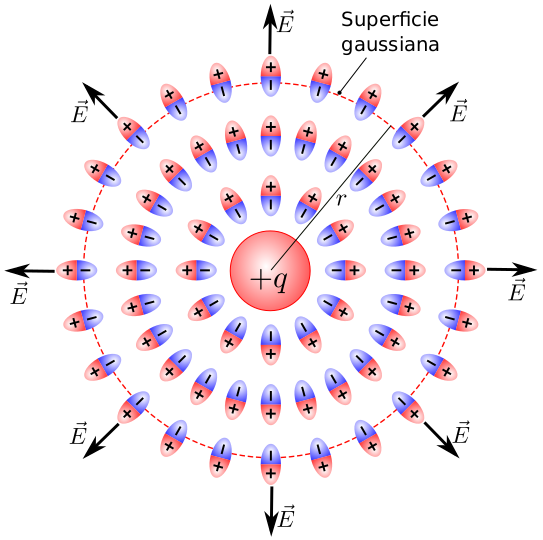
\includegraphics[scale = 0.55]{Figuras/Ej-Isotropico.png}
        \caption{Carga en un medio dieléctrico. 
 Recuperado de \cite{Alvarez} en la pág. 128. }
        \label{fig:Carga-Dielectrico}
    \end{figure}

    \textbf{Solución:} Si suponemos que el material es lineal e isotrópico, los vectores $\Vec{E}$, $\Vec{D}$ y $\Vec{P}$ son paralelos. Por simetría esférica, el campo eléctrico es radial, así que
    $$\Vec{D} = D(r)  \,\hat{r}, \quad \Vec{E} = E(r) \,\hat{r}, \quad \Vec{P} = P(r) \,\hat{r}.$$

    Usando la ley de Gauss para una superficie gaussiana esférica de radio $r$ con origen en la carga $q$,
    \begin{align*}
       \oiint_S \Vec{D} \cdot d\Vec{S} &= q_{libre} \\
       \int_0^{\pi} \int_0^{2\pi} (D(r) \,\hat{r}) \cdot (r^2 \sin \theta \,d\varphi \,d\theta) &= q \\
       4\pi r^2 D(r) &= q \\
       D(r) &= \frac{q}{4\pi r^2}.
    \end{align*}

    Entonces,
    $$\Vec{D} = \frac{q}{4\pi r^2} \,\hat{r}.$$

    El campo eléctrico se obtiene de $\Vec{D} = \varepsilon \Vec{E} = \kappa \varepsilon_0 \Vec{E}$,
    $$\Vec{E} = \frac{q}{4\pi \kappa \varepsilon_0 r^2} \,\hat{r}.$$

    Por último, el vector de polarización está dado por
    $$\Vec{P} = (\kappa -1) \varepsilon_0 \Vec{E} = \frac{(\kappa-1)q}{4\pi \kappa r^2} \,\hat{r}.$$
\end{ejemplo}

\subsection{Condiciones de borde*} \label{sec:Cond-Borde-Dielectricos}

Consideremos dos dieléctricos separados por una superficie de frontera, ver figura \ref{fig:Borde-Normal}. Queremos saber como cambian los vectores $\Vec{E}$ y $\Vec{D}$ cuando estos cruzan la frontera. 

\begin{figure}[H]
    \centering
    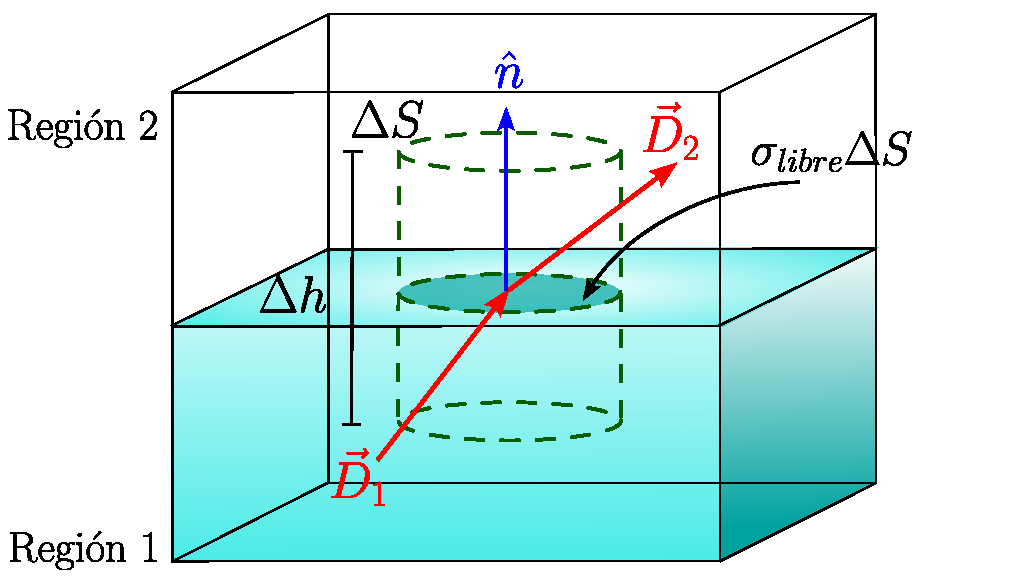
\includegraphics[scale = 0.6]{Figuras/Condicion-Borde-Normal.pdf}
    \caption{Condición de borde para la componente normal.}
    \label{fig:Borde-Normal}
\end{figure}

Si ampliamos la superficie, ésta se aproximará a un plano de tal forma que la densidad de carga (libre) y $\Vec{D}$ sean constantes. Aplicamos la ley de Gauss usando como superficie $S$ el cilindro de la figura \ref{fig:Borde-Normal}. 
$$\oiint_S \Vec{D} \cdot d\Vec{S} = q_{libre}.$$

Como $\sigma_{libre}$ se puede considerar constante, la carga libre encerrada $q_{libre} = \sigma_{libre} \Delta S$, luego separando las superficies que constituyen el cilindro,
\begin{equation}
\iint_{S_1} \Vec{D}_1 \cdot d\Vec{S} + \iint_{S_2} \Vec{D}_2 \cdot d\Vec{S} + \iint_{S_3} \Vec{D} \cdot d\Vec{S} = \sigma_{libre} \Delta S,    \label{Borden-Normal}
\end{equation}

donde $S_1$ es la tapa inferior, $S_2$ la tapa superior y $S_3$ el manto del cilindro. 

Ahora, si $\Delta h \to 0$, la integral $\int_{S_3} \Vec{D} \cdot d\Vec{S}$, que es proporcional a $\Delta h$, se anula en este límite. Además, si consideramos $\hat{n}$ el vector unitario normal a la superficie que apunta desde la región 1 hasta la región 2, la ecuación \eqref{Borden-Normal} nos queda:
\begin{align*}
    -(\Vec{D}_1 \cdot \hat{n}) \iint_{S_1} dS + (\Vec{D}_2 \cdot \hat{n}) \iint_{S_2} dS &= \sigma_{libre} \Delta S \\
    -(\Vec{D}_1 \cdot \hat{n}) \Delta S + (\Vec{D}_2 \cdot \hat{n}) \Delta S &= \sigma_{libre} \Delta S \\
    -(\Vec{D}_1 \cdot \hat{n}) + (\Vec{D}_2 \cdot \hat{n}) &= \sigma_{libre}.
\end{align*}

Por lo tanto,
\begin{shaded}
\begin{equation}
  \Vec{D}_2 \cdot \hat{n} - \Vec{D}_1 \cdot \hat{n} = \sigma_{libre}.  \label{Componente-Normal}
\end{equation}
\end{shaded}

La expresión \eqref{Componente-Normal} nos quiere decir que la componente normal de $\Vec{D}$ es discontinua en una interfase entre dos dieléctricos siempre y cuando exista una carga superficial.

\textbf{Observación:} Si los medios son lineales e isotrópicos $\Vec{D} = \varepsilon \Vec{E}$ y las regiones 1 y 2 tienen permitividades $\varepsilon_1$ y $\varepsilon_2$, respectivamente, se cumple
$$\varepsilon_2 \Vec{E}_2 \cdot \hat{n} - \varepsilon_1 \Vec{E}_1 \cdot \hat{n} = \sigma_{libre}.$$

Para el vacío, $\varepsilon_1 = \varepsilon_2 = \varepsilon_0$
$$\Vec{E}_2 \cdot \hat{n} - \Vec{E}_1 \cdot \hat{n} = \frac{\sigma}{\varepsilon_0},$$

donde hemos denotado $\sigma_{libre}$ simplemente como $\sigma$.

Por otro lado, estudiemos qué sucede con la componente tangencial del campo eléctrico. 

\begin{figure}[H]
    \centering
    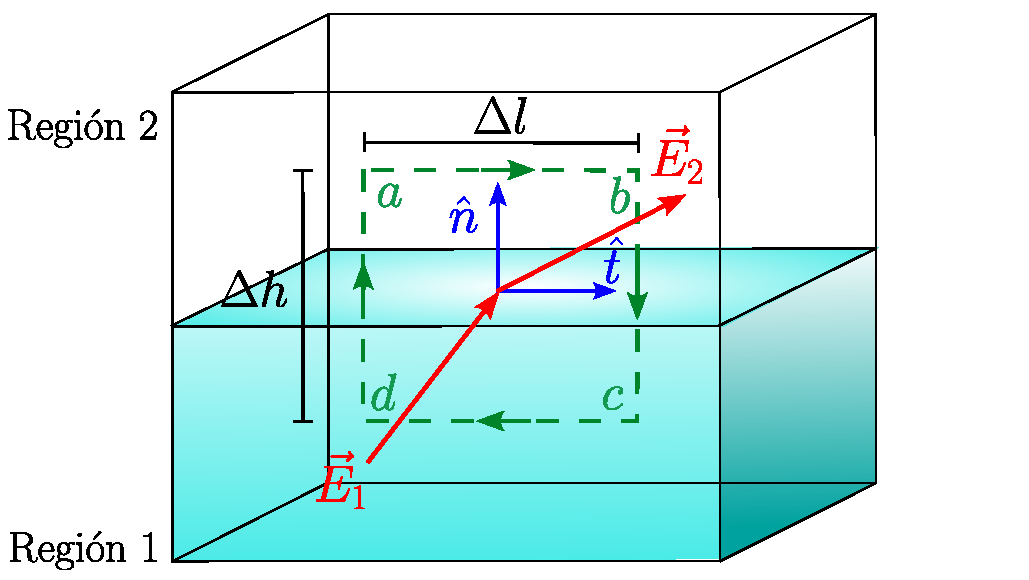
\includegraphics[scale = 0.6]{Figuras/Condicion-Borde-Tangencial.pdf}
    \caption{Condición de borde para la componente tangencial.}
    \label{fig:Borde-Tangencial}
\end{figure}

Como el campo eléctrico es conservativo (en electrostática), la integral de línea siguiendo cualquier curva cerrada es cero. En nuestro caso elegimos el camino rectangular $abcd$ de la figura \ref{fig:Borde-Tangencial}.
$$\oint_{abcd} \Vec{E} \cdot \,d\Vec{x} = 0.$$

 Descomponemos la trayectoria en los segmentos $ab$, $bc$, $cd$ y $da$:
\begin{equation}
\int_{ab} \Vec{E} \cdot d\Vec{x} + \int_{bc} \Vec{E} \cdot d\Vec{x} + \int_{cd} \Vec{E} \cdot d\Vec{x} + \int_{da} \Vec{E} \cdot d\Vec{x} = 0.   \label{Borden-Tangencial}
\end{equation}

Ahora, si $\Delta h \to 0$, las integrales $\int_{bc} \Vec{E} \cdot d\Vec{x}$ y  $\int_{da} \Vec{E} \cdot d\Vec{x}$, que son proporcionales a $\Delta h$, se anula en este límite. Además, si consideramos $\hat{t}$ un vector tangencial a la superficie que apunta en el mismo sentido que el segmento $ab$, la ecuación \eqref{Borden-Tangencial} nos queda:
\begin{align*}
    (\Vec{E}_2 \cdot \hat{t}) \int_{ab} dx - (\Vec{E}_1 \cdot \hat{t}) \int_{cd} dx &= 0 \\
    (\Vec{E}_2 \cdot \hat{t}) \Delta l - (\Vec{E}_1 \cdot \hat{t}) \Delta l &= 0 .
\end{align*}

Por lo tanto, 
\begin{shaded}
\begin{equation}
    \Vec{E}_2 \cdot \hat{t} = \Vec{E}_1 \cdot \hat{t}.    \label{Componente-Tangencial}
\end{equation}
\end{shaded}

Dado que la dirección del vector $\hat{t}$ es arbitraria (pero siempre tangencial a la superficie), la condición \eqref{Componente-Tangencial} implica que las componentes tangenciales (2 componentes linealmente independientes) del campo eléctrico permanecen inalteradas al cruzar la superficie, es decir, la componente tangencial del campo eléctrico es continua.

\begin{ejemplo} \label{Ej-Cond-Borde}
Una esfera conductora de radio $R$ flota hasta la mitad en un medio dieléctrico de permitividad eléctrica $\varepsilon_1$. La región sobre la esfera es un gas de permitividad eléctrica $\varepsilon_2$. La esfera está carga con una carga igual a $Q$.

\begin{figure}[H]
    \centering
    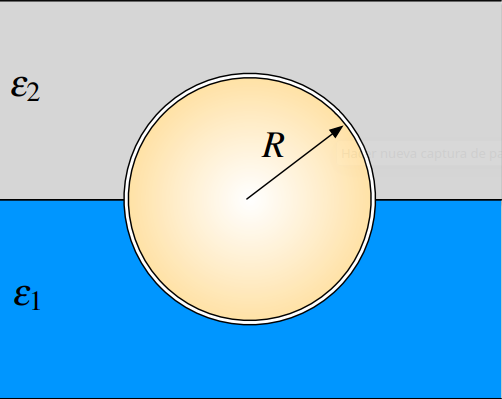
\includegraphics[scale = 0.45]{Figuras/Ej-Condicion-Borde.png}
    \caption{Esfera conductora sumergida en dos dieléctricos.}
    \label{fig:Ej-Condicion-Borde}
\end{figure}

\begin{itemize}
    \item[(a)] Calcule el campo eléctrico en todo el espacio. 

    \item[(b)] Calcule la densidad de carga libre superficial en la esfera conductora, y la densidad superficial de carga de polarización de ambos medios dieléctricos en la interfaz con la esfera.
\end{itemize}

\textbf{Solución:} Primero elegimos un sistema coordenado como el de la figura \ref{fig:Ej-Condicion-Borde-1}.

\begin{figure}[H]
    \centering
    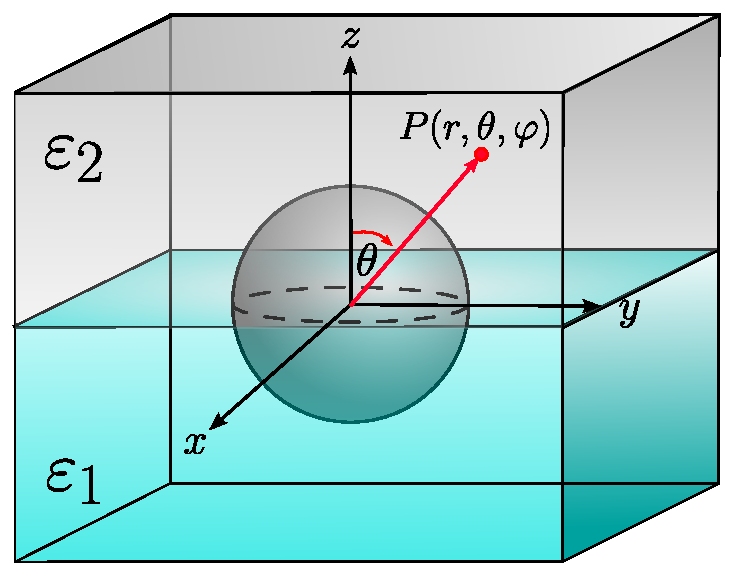
\includegraphics[scale = 0.6]{Figuras/Ej-Condicion-Borde.pdf}
    \caption{Sistema coordenado.}
    \label{fig:Ej-Condicion-Borde-1}
\end{figure}

\begin{itemize}
    \item[(a)] Para $r < R$, se tiene que $\Vec{E} = \Vec{0}$ ya que es un conductor. Para $r > R$, usaremos la ley de Gauss, teniendo en cuenta que $\Vec{D} = D(r) \,\hat{r}$ y la superficie Gaussiana $S$ esférica de radio $r$ centrada en la esfera conductora. Así,
    $$\oiint_S \Vec{D} \cdot d\Vec{S} =  q_{libre} \Rightarrow \int_0^{\pi} \int_0^{2\pi} D(r) r^2 \sin \theta \,d\varphi \,d\theta = Q.$$

    Si $\Vec{D}_1$ y $\Vec{D}_2$ son los vectores de desplazamiento de los dieléctricos con permitividad eléctrica  $\varepsilon_1$ y $\varepsilon_2$, respectivamente, tenemos que
    \begin{align*}
     \int_0^{\pi/2} \int_0^{2\pi} D_2(r) r^2 \sin \theta \,d\varphi \,d\theta + \int_{\pi/2}^{\pi} \int_0^{2\pi} D_2(r) r^2 \sin \theta \,d\varphi \,d\theta &= Q\\
    \Rightarrow \quad D_2(r) \cdot 2\pi r^2 + D_1(r) \cdot 2\pi r^2 &= Q.   
    \end{align*}

    Ahora, debido a la simetría, el campo eléctrico es completamente tangente a la interfase de los medios, ver figura \ref{fig:Ej-Condicion-Borde-2}. Entonces, $\Vec{E}_1 = \Vec{E}_2 = \Vec{E}$. Además, $D_1(r) = \varepsilon_1 E(r)$ y $D_2(r) = \varepsilon_2 E(r)$. Por lo tanto, el campo eléctrico, para $r > R$, está dado por
    $$\Vec{E}(r) = \frac{Q}{2\pi r^2(\varepsilon_1 + \varepsilon_2)} \,\hat{r}.$$

    \begin{figure}[H]
    \centering
    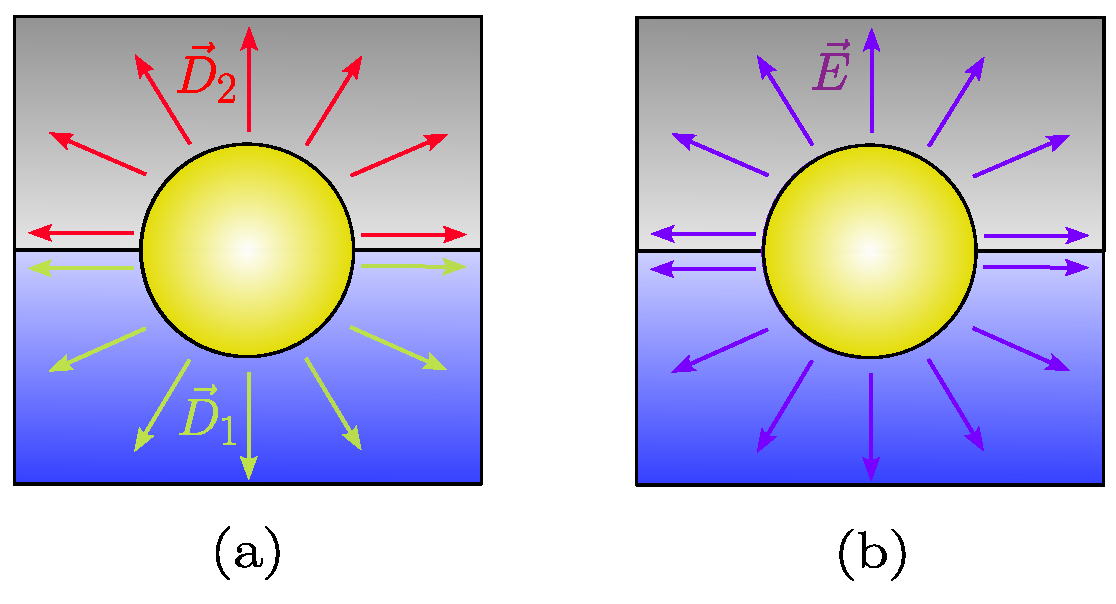
\includegraphics[scale = 0.6]{Figuras/Ej-Condicion-Borde-2.pdf}
    \caption{Vectores de desplazamiento (a) y el campo eléctrico (b) de una esfera sumergida en dos dieléctricos.}
    \label{fig:Ej-Condicion-Borde-2}
\end{figure}
    
    \item[(b)] La densidad de carga libre dependerá del hemisferio de la esfera. Entonces, para el hemisferio inferior:
    $$\sigma_{l1} = \left.\vec{D}_1(r) \cdot \hat{n} \right|_{r = R} = \frac{\varepsilon_1Q}{2\pi R^2(\varepsilon_1 + \varepsilon_2)} \hat{r} \cdot \hat{r} = \frac{\varepsilon_1Q}{2\pi R^2(\varepsilon_1 + \varepsilon_2)}$$

    y para el hemisferio superior:
     $$\sigma_{l2} = \left.\vec{D}_2(r) \cdot \hat{n} \right|_{r = R} = \frac{\varepsilon_2Q}{2\pi R^2(\varepsilon_1 + \varepsilon_2)} \hat{r} \cdot \hat{r} = \frac{\varepsilon_2Q}{2\pi R^2(\varepsilon_1 + \varepsilon_2)}.$$

     Por otro lado, para calcular las cargas de polarización debemos primero determinar el vector de polarización en cada medio. Para ello, recordemos que
     $$\Vec{D} = \varepsilon_0 \Vec{E} + \Vec{P} = \varepsilon \Vec{E} \Rightarrow \vec{P} = (\varepsilon - \varepsilon_0) \Vec{E}.$$

     Así, para el medio de permitividad $\varepsilon_1$,
     $$\Vec{P}_1 = (\varepsilon_1 - \varepsilon_0) \Vec{E} = \frac{(\varepsilon_1 - \varepsilon_0)Q}{2\pi r^2(\varepsilon_1 + \varepsilon_2)} \,\hat{r}.$$

     Luego,
     $$\sigma_{p1} = \left.\vec{P}_1(r) \cdot \hat{n} \right|_{r = R} = \frac{(\varepsilon_1 - \varepsilon_0) Q}{2\pi R^2(\varepsilon_1 + \varepsilon_2)} \hat{r} \cdot (-\hat{r}) = - \frac{(\varepsilon_1 - \varepsilon_0)Q}{2\pi R^2(\varepsilon_1 + \varepsilon_2)}.$$

     Análogamente,
     $$\sigma_{p2}  = - \frac{(\varepsilon_2 - \varepsilon_0)Q}{2\pi R^2(\varepsilon_1 + \varepsilon_2)}.$$

     Notar el hecho que el vector unitario normal en el caso de la densidad de carga libre apunta desde el conductor al dieléctrico y en el caso de la densidad de carga de polarización apunta en el sentido inverso.
\end{itemize}

\end{ejemplo}

\subsection{La ecuación de Poisson y Laplace en un medio dieléctrico*}

Si el medio dieléctrico es lineal isotrópico y homogéneo, de la ley de Gauss, $\Vec{\nabla} \cdot \Vec{D} = \rho$, $\Vec{D} = \varepsilon \Vec{E}$ y de $\Vec{E} = - \Vec{\nabla} \phi$, 
\begin{shaded}
    $$\nabla^2 \phi = -\frac{\rho}{\varepsilon}.$$
\end{shaded}

Por otro lado, la ecuación de Laplace queda idéntica a la del vacío 
\begin{shaded}
    $$\nabla^2 \phi = 0.$$
\end{shaded}

\begin{ejemplo}
Dos conductores esféricos concéntricos de radios $a$ y $b$, con $a < b$, están separados por un dieléctrico cuya constante varía según la ley:
$$\varepsilon(r) = \frac{c+r}{r},$$

donde $r$ es la distancia al centro común de las dos esferas conductoras. Si la esfera interior está aislada y lleva carga $Q$, considerando que la esfera exterior está conectada a tierra. Encuentre el potencial eléctrico en el dieléctrico.

\textbf{Solución:} Dado que entre los conductores no hay carga, $\rho_{libre} = 0$, y por la ley de Gauss, se satisface:
\begin{equation}
 \Vec{\nabla} \cdot \Vec{D} = 0.   \label{Ej-Laplace-1}
\end{equation}

Considerando el dieléctrico como un medio lineal e isotrópico, $\Vec{D} = \varepsilon \Vec{E}$, pero en este caso $\varepsilon$ es una función de radio, así que el medio no es homogéneo. Luego,
$$\Vec{D} = \varepsilon(r) \Vec{E} = \left( \frac{c+r}{r} \right) \Vec{E} = \left( \frac{c+r}{r} \right) \left( - \Vec{\nabla} \phi\right).$$

\begin{figure}[H]
    \centering
    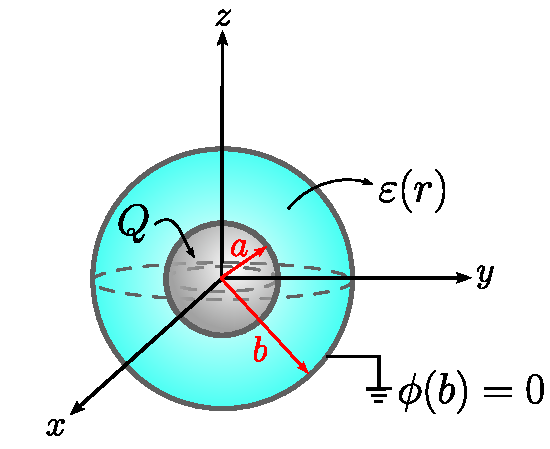
\includegraphics[scale = 0.8]{Figuras/Ej-Laplace-Dielectric.pdf}
    \caption{Capacitador conectado a tierra rellenado con un dieléctrico de permitividad eléctrica $\varepsilon(r)$.}
    \label{fig:Ej-Laplace-Dielectric}
\end{figure}

El problema presenta simetría axial y azimutal (es decir, esférica), por lo que $\phi = \phi(r)$. En coordenadas esféricas,
$$\Vec{\nabla} \phi(r) = \frac{d \phi(r)}{d r}\,\hat{r}.$$

Reemplazando en \eqref{Ej-Laplace-1},
\begin{align*}
    \Vec{\nabla} \cdot \left( - \left( \frac{c+r}{r} \right) \frac{d \phi}{d r} \,\hat{r}\right) &= 0 \\
    \frac{1}{r^2} \frac{d}{d r} \left[ r^2 \left( - \frac{c+r}{r} \frac{d \phi}{d r} \right)\right] &= 0 \\
    \frac{d}{dr} \left[- r(c+r) \frac{d \phi}{dr} \right] &= 0 \\
    (cr + r^2) \frac{d\phi}{dr} &= -A \\
    \frac{d\phi}{dr} &= - \frac{A}{cr+r^2},
\end{align*}

donde $A$ es una constante de integración. Integrando con respecto a $r$:
\begingroup
\allowdisplaybreaks
\begin{align*}
    \phi(r) &= \int - \frac{A}{cr+r^2} \,dr + B \\
    &= A \left(  \int \frac{1}{c(c+r)} \,dr - \int \frac{1}{cr} \,dr \right) + B \\
    &= A \left( \frac{1}{c}\ln(c+r) - \frac{1}{c} \ln(r) \right) + B \\
    &= \frac{A}{c} \ln\left(\frac{c+r}{r} \right) + B, \quad a \leq r \leq b.
\end{align*}
\endgroup

Para encontrar las constante de integración $A$ y $B$, debemos evaluar las condiciones de borde:
\begin{itemize}
    \item $(\Vec{D}_2 - \Vec{D}_1) \cdot \hat{n}|_{r = a} = \sigma_{libre}$.
    
    \item $\phi(b) = 0$, pues el conductor externo está conectado a tierra.
\end{itemize}

Si la carga $Q$ está distribuida uniformemente, 
$$\sigma_{libre} = \frac{Q}{4\pi a^2}.$$

En $r = a$, $\Vec{D}_1 = \Vec{0}$, entonces la primera condición de borde nos queda:
$$\Vec{D}_2 = \varepsilon \Vec{E}|_{r=a} \cdot \hat{n} = - \varepsilon(r) \Vec{\nabla} \phi|_{r = a}  \cdot \hat{r} = \sigma_{libre}.$$

Aplicando el gradiente en coordenadas esféricas, 
$$-\varepsilon(r) \left. \frac{\partial \phi}{\partial r} \right|_{r = a} =\frac{Q}{4\pi a^2}.$$

Calculando
$$\frac{\partial \phi}{\partial r} =  \frac{A}{c} \frac{\partial}{\partial r} \left[\ln\left(\frac{c+r}{r}  \right) \right] = - \frac{A}{r(c+r)}.$$

Entonces,
$$-\varepsilon(r) \left. \frac{\partial \phi}{\partial r} \right|_{r = a} =  \frac{c+a}{a} \cdot \frac{A}{a(c+a)} = \frac{Q}{4\pi a^2} \Rightarrow A = \frac{Q}{4\pi}.$$

Así,
$$\phi(r) = \frac{Q}{4\pi c} \ln\left(\frac{c+r}{r} \right) + B, \quad a \leq r \leq b.$$

Ahora, si imponemos $\phi(b) = 0$, tenemos que 
$$\frac{Q}{4\pi c} \ln\left(\frac{c+b}{b} \right) + B = 0 \Rightarrow B = - \frac{Q}{4\pi c} \ln\left(\frac{c+b}{b} \right).$$

Por lo tanto,
$$\phi(r) =  \frac{Q}{4\pi c} \ln \left\{\left( \frac{b}{r}\right) \left( \frac{c+r}{c+b}\right) \right\}, \quad a \leq r\leq b.$$
\end{ejemplo}

\subsection{Energía electrostática en términos de \texorpdfstring{$\Vec{E}$}{TEXT} y \texorpdfstring{$\Vec{D}$}{TEXT}*}

Recordemos que la energía electrostática de una distribución continua de cargas está dada por
$$U = \frac{1}{2} \iiint_{V} \rho \phi(\Vec{x}) \,dV.$$

Si sustituimos $\rho = \Vec{\nabla} \cdot \Vec{D}$,
$$U = \frac{1}{2} \iiint_{V} (\Vec{\nabla} \cdot \vec{D}) \phi(\Vec{x}) \,dV.$$

Usando la identidad 
$$\Vec{\nabla}\cdot (\phi \Vec{D}) = \phi \Vec{\nabla} \cdot \Vec{D} + \Vec{D} \cdot \Vec{\nabla} \phi,$$

tenemos que
$$U = \frac{1}{2} \iiint_{V} (\Vec{\nabla}\cdot (\phi \Vec{D}) -  \Vec{D} \cdot \Vec{\nabla} \phi) \,dV = \frac{1}{2} \iiint_{V} \Vec{\nabla} \cdot (\phi \Vec{D}) \,dV - \frac{1}{2} \iiint_{V} \Vec{D} \cdot \Vec{\nabla} \phi \,dV.$$

En la primera integral usamos el teorema de Gauss y en la segunda sustituimos $\Vec{\nabla} \phi = - \Vec{E}$.
$$U = \frac{1}{2} \oiint_{S} \phi \Vec{D} \cdot d\Vec{S} + \frac{1}{2} \iiint_{V} \Vec{D} \cdot \Vec{E} \,dV.$$

La superficie $S$ puede ser cualquiera que rodee a las cargas, por lo tanto podemos elegir una esfera de radio $R$. Cuando se toma el límite $R \to \infty$, el potencial disminuye a razón de $1/R$ mientras que el desplazamiento disminuye a razón $1/R^2$. Por otro lado, la superficie $S$ aumenta a razón $R^2$. Es decir, la primera integral disminuye a razón $1/R$ y se hará cero a medida que $R \to \infty$. De esta manera podemos despreciar la integral de superficie y escribir:
\begin{shaded}
    $$U = \frac{1}{2} \iiint_{\mathbb{R}^3} \Vec{D} \cdot \Vec{E} \,dV.$$
\end{shaded}

Para un medio lineal e isótropo $\Vec{D} = \varepsilon \Vec{E}$,
\begin{shaded}
    $$U = \frac{1}{2} \iiint_{\mathbb{R}^3} \varepsilon \Vec{E}^2\,dV.$$
\end{shaded}

\begin{ejemplo}
    Calcule la energía almacenada en el campo eléctrico en el ejemplo \ref{Ej-Cond-Borde}.

    \textbf{Solución:} En el ejemplo \ref{Ej-Cond-Borde} encontramos que el campo eléctrico estaba dado por
    $$\vec{E}(r) = \left\{ \begin{array}{cl}
        \Vec{0}, & \text{si} ~ r < R  \\
         \frac{Q}{2\pi r^2 (\varepsilon_1 + \varepsilon_2)} \,\hat{r},& \text{si} ~ r > R 
    \end{array} \right. .$$

    Además, 
    $$\varepsilon = \left\{ \begin{array}{cl}
        0, & \text{si} ~ r < R  \\
         \varepsilon_2, & \text{si} ~ r > R ~\wedge~ 0 \leq \theta < \pi/2 \\ 
          \varepsilon_1, & \text{si} ~ r > R ~\wedge~ \pi/2 \leq \theta < \pi
    \end{array} \right. .$$

    Por lo tanto, la energía almacenada en el campo eléctrico es
    \begin{align*}
        U &= \frac{1}{2} \iiint_{\mathbb{R}^3} \varepsilon \Vec{E}^2 \,dV \\
        &= \frac{1}{2} \left\{ \int_R^{\infty} \int_0^{\pi/2} \int_0^{2\pi}  \frac{\varepsilon_2 Q^2}{4\pi^2 r^4 (\varepsilon_1 + \varepsilon_2)^2}   r^2 \sin \theta \,d\varphi \,d\theta \,dr \right. \\
        &\left. \quad + \int_R^{\infty} \int_{\pi/2}^{\pi} \int_0^{2\pi}   \frac{\varepsilon_1 Q^2}{4\pi^2 r^4 (\varepsilon_1 + \varepsilon_2)^2}  r^2 \sin \theta \,d\varphi \,d\theta \,dr  \right\} \\
        &= \frac{Q^2}{8\pi^2 (\varepsilon_1 + \varepsilon_2)^2} \left\{ 2\pi \varepsilon_2 \int_R^{\infty} \frac{1}{r^2} \int_0^{\pi/2} \sin \theta \,d\theta \,dr +  2\pi \varepsilon_1 \int_R^{\infty} \frac{1}{r^2} \int_{\pi/2}^{\pi} \sin \theta \,d\theta \,dr \right\} \\
        &= \frac{Q^2}{8\pi^2 (\varepsilon_1 + \varepsilon_2)^2} \left\{ 2\pi \varepsilon_2 \int_R^{\infty} \frac{1}{r^2} \,dr +  2\pi \varepsilon_1 \int_R^{\infty} \frac{1}{r^2} \,dr \right\} \\
        &= \frac{Q^2}{8\pi^2 (\varepsilon_1 + \varepsilon_2)^2} \cdot \frac{2\pi}{R} (\varepsilon_1 + \varepsilon_2) \\
        &= \frac{Q^2}{4\pi R (\varepsilon_1 + \varepsilon_2)}.
    \end{align*}
\end{ejemplo}